\documentclass[letterpaper,twocolumn,openany,nodeprecatedcode]{dndbook}

% Use babel or polyglossia to automatically redefine macros for terms
% Armor Class, Level, etc...
% Default output is in English; captions are located in lib/dndstring-captions.sty.
% If no captions exist for a language, English will be used.
%1. To load a language with babel:
%	\usepackage[<lang>]{babel}
%2. To load a language with polyglossia:
%	\usepackage{polyglossia}
%	\setdefaultlanguage{<lang>}
\usepackage[italian]{babel}
%\usepackage[italian]{babel}
% For further options (multilanguage documents, hypenations, language environments...)
% please refer to babel/polyglossia's documentation.

\usepackage[utf8]{inputenc}
\usepackage[singlelinecheck=false]{caption}
\usepackage{lipsum}
\usepackage{listings}
\usepackage{shortvrb}
\usepackage{stfloats}
\usepackage{titling}
\usepackage{multicol}
\usepackage{hyperref}
\usepackage{pdfpages}
\usepackage{lscape} 


\captionsetup[table]{labelformat=empty,font={sf,sc,bf,},skip=0pt}

\MakeShortVerb{|}

\lstset{%
  basicstyle=\ttfamily,
  language=[LaTeX]{TeX},
  breaklines=true,
}

\pretitle{%
  \begin{center}
  \LARGE
    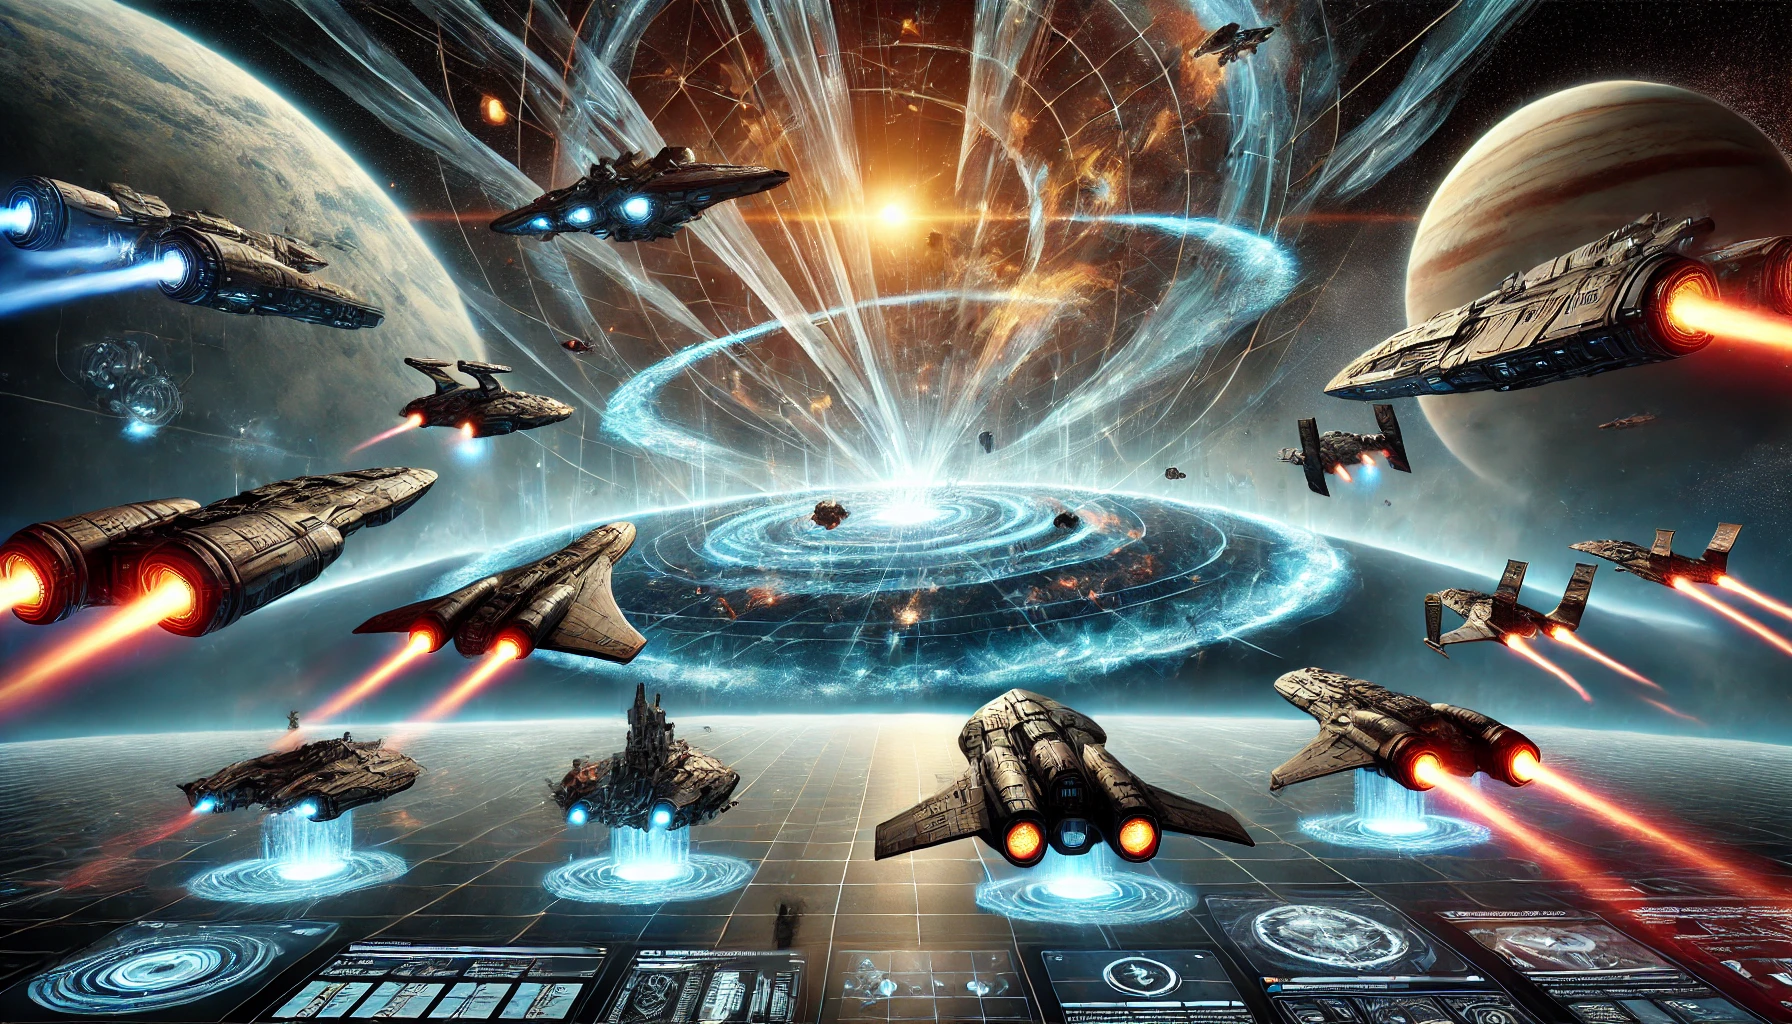
\includegraphics[width=1\linewidth]{header_multitavolo.jpg}
}
\posttitle{\end{center}}
    
\title{Figures of a future past}

\author{Marco Montanari\\
\textit{(Just Play Bologna, Mensa Italia)}\\
Edoardo Lascialfari\\
\textit{(Mensa Italia)}\\
Emlio Marco Tonoli\\
\textit{(Mensa Italia)}\\
\date{2025}
}

\newlist{todolist}{itemize}{2}
\setlist[todolist]{label=$\square$}
\usepackage{pifont}
\newcommand{\cmark}{\ding{51}}%
\newcommand{\xmark}{\ding{55}}%
\newcommand{\done}{\rlap{$\square$}{\raisebox{2pt}{\large\hspace{1pt}\cmark}}%
\hspace{-2.5pt}}
\newcommand{\wontfix}{\rlap{$\square$}{\large\hspace{1pt}\xmark}}


\makeatletter
\renewcommand{\@chapapp}{}
\makeatother



\begin{document}



\frontmatter

\maketitle

\tableofcontents

\mainmatter%

\chapter{Introduzione}

\DndDropCapLine{B}{envenuti all’avventura multitavolo} "Immagini da un passato futuro"! Questo manuale fornisce ai Master le linee guida necessarie per condurre l’avventura multitavolo. 

Situata nel sistema Tartarus, l’anomalia subspaziale e l’artefatto iconiano rappresentano il fulcro della storia. Ogni tavolo simula una nave diversa con obiettivi, risorse e motivazioni specifiche. Come Master, la vostra responsabilità è orchestrare gli eventi, garantendo che le decisioni dei giocatori abbiano un impatto significativo sulla narrativa globale e sui destini di interi pianeti.

\section{Premessa Narrativa}

Nel sistema Tartarus, ai limiti della regione della Shackleton Expanse a poche centinaia di anni luce da Narendra Station, è stata scoperta un’anomalia subspaziale che emette segnali iconiani, una tecnologia appartenente a una civiltà scomparsa improvvisamente centinaia di migliaia di anni fa. Gli Iconiani, leggendari per i loro portali in grado di connettere mondi distanti istantaneamente, hanno lasciato dietro di sé solo frammenti della loro avanzata tecnologia. Tuttavia, questa scoperta ha riattivato qualcosa di molto più pericoloso: un artefatto iconiano che minaccia di risvegliare una rete di portali in tutta la galassia.

Ogni fazione coinvolta nell’avventura ha obiettivi unici e motivazioni che guidano le loro azioni:

\begin{itemize}
    \item \textbf{La Federazione} (\textit{Star Trek Adventures}): Esplorare e proteggere l'artefatto iconiano, prevenendo l’abuso della tecnologia iconiana da parte di altre fazioni.
    \item \textbf{I Ferengi e i Romulani} (\textit{Scum and Villainy}): Cercare ricchezza e vantaggi strategici, con una fragile alleanza tra avidità e sospetto reciproco.
    \item \textbf{La SS Halcyon} (\textit{Mothership}): Sopravvivere agli effetti devastanti dell’anomalia e proteggere il proprio pianeta natale dalla distruzione.
    \item \textbf{L’HSS Ironclad} (\textit{Death in Space/Alien}): Neutralizzare la minaccia iconiana e garantire la sicurezza dei pianeti dell’Alleanza, anche a costo di sacrifici estremi.
\end{itemize}

Queste diverse prospettive creano tensioni naturali che possono sfociare in conflitti o in alleanze instabili.

L’anomalia non è solo una reliquia del passato: è un sistema iconiano semi-intelligente che manipola attivamente segnali e visioni. Questa "intelligenza incomprensibile" osserva le azioni delle fazioni e agisce di conseguenza, rendendo le intenzioni dell’artefatto un mistero da decifrare. I Master devono utilizzare questo elemento per introdurre dubbi e tensione, incentivando i giocatori a collaborare o a competere in modo strategico. Le vostre decisioni determineranno il destino della galassia.



\section{ Obiettivi Globali
}

\begin{enumerate}
    \item Scoprire la natura dell’anomalia: Cosa è il frammento iconiano e perché si sta riattivando?
    \item Gestire i portali: Stabilizzare, distruggere o attivare la rete iconiana?
    \item Proteggere i pianeti d’origine: Ogni fazione rischia che i portali si connettano a pianeti chiave, causando devastazione.
    \item Collaborare o competere: Decidete se cooperare per un obiettivo comune o agire secondo gli interessi della vostra fazione.
\end{enumerate}



\section{ Elementi Chiave della Storia
}

\subsection{ L’Anomalia Subspaziale
}

Un fenomeno che altera le comunicazioni e i sensori, rendendo difficile la collaborazione tra le navi. I segnali emessi contengono frammenti di informazioni iconiane, ma sono disturbati e incompleti. Ad esempio, un messaggio inviato da una nave potrebbe arrivare frammentato o alterato, con parole sostituite da simboli iconiani incomprensibili. Questo costringe i giocatori a interpretare e ricostruire il contenuto, aumentando la tensione e il senso di isolamento.


\subsubsection{ I Portali Iconiani
}

Una rete dormiente che si sta riattivando. Ogni portale può connettersi a un pianeta o a un punto dello spazio. La loro riattivazione incontrollata potrebbe devastare mondi o aprire passaggi verso luoghi sconosciuti.

\subsection{ L’Intelligenza Incomprensibile
}

Un frammento dell’antico sistema iconiano agisce come un osservatore o manipolatore. I suoi messaggi sono criptici e frammentari, costringendo i giocatori a interpretare le sue intenzioni.



\section{ Struttura dell’Avventura
}

\paragraph{1. Introduzione (15 minuti)}

   Ogni tavolo riceve un briefing sulla propria missione iniziale e sulla situazione nel sistema Tartarus.
   I giocatori si ambientano nei loro ruoli e discutono le strategie iniziali.

\paragraph{2. Missioni Iniziali (60 minuti)}

   Ogni tavolo affronta una sfida specifica legata alla loro fazione e riceve frammenti di informazioni sull’anomalia.
   Le prime comunicazioni tra tavoli iniziano a emergere negli ultimi 10 minuti della fase

\paragraph{3. Svolta (90 minuti)}

   L’anomalia si intensifica e un portale si attiva parzialmente, minacciando un pianeta chiave.
   I tavoli devono collaborare per decifrare i segnali iconiani o affrontare le conseguenze da soli.

\paragraph{4. Conclusione (75 minuti)}

   La scelta finale: stabilizzare, distruggere o attivare il portale.
   Ogni tavolo contribuisce al risultato globale, con possibili alleanze o conflitti.

\section{ Strumenti e Meccaniche di Gioco
}

\subsection{ Comunicazioni Limitate
}

Le comunicazioni tra tavoli sono ritardate o disturbate a causa dell’anomalia. I messaggi devono passare attraverso il Master Generale e possono arrivare incompleti.

\subsection{ Risorse Condivise
}

Alcune risorse chiave (es. frammenti dell’artefatto) devono essere scambiate o condivise tra i tavoli per progredire.

\subsection{ Eventi Globali
}

Il Master Generale annuncia eventi globali che influenzano tutti i tavoli (es. una nuova attivazione del portale o un collasso subspaziale).

\section {Interazoni fra navi}
Essendo ogni tavolo governato da regole proprie, ed essendo l'avventura basata molto su una serie di elementi, per fare un attacco fra le navi verrà utilizzato un sistema di calcolo custom, chiamato "Convergenza Iconiana", basato sui vari modificatori signficativi del gioco. 

In generale il tiro di convergenza si basa sul tiro di 2d6 come riferimento centrale, a seguito di un tentativo di negoziazione e di interazione. 


\section{Conclusione}

Ogni tavolo avrà un ruolo cruciale nel determinare il finale dell’avventura. Le decisioni dei giocatori influenzeranno direttamente il destino dei loro pianeti natali, della rete iconiana e delle relazioni interstellari. I Master dovranno assicurarsi che ogni scelta porti a conseguenze tangibili, creando una narrativa epica e coerente. Siete pronti ad affrontare il ritorno degli Iconiani?

\chapter {Fasi}
\section{Introduzione (15 minuti)}
In questa fase introduziamo i personaggi, il feeling della giocata e le regole generali ai giocatori. Il dettaglio verrà dato nei capitoli specifici delle varie fazioni. Non si va ancora a parlare dei \textit{Quantum Data Points}, che saranno poi la risorsa con cui i vari gruppi potranno interagire fra loro e con l'anomalia. 
\section {Missione iniziale (60 minuti)}
In questa fase viene data al tavolo la prima missione generale che porterà i giocatori a familiarizzare con lo strumento mentre si avvicinano all'anomalia che sarà il leitmotiv delle ore successive. 
\section {Svolta (90 minuti)}
Le interazioni fra navi e con l'anomalia diventano sempre più frequenti e richiedono coordinamento complesso. Ogni tipologia di interazione fa guadagnare e perdere QDP di vario tipo
\section {Conclusione (60 minuti)}

\section {Concilio Iconiano (15 minuti)}

\subsection{Premessa}
Durante la fase conclusiva, quando l'artefatto iconiano raggiunge il punto critico di attivazione, si manifesta una connessione diretta che permette a un rappresentante di ciascuna nave di essere fisicamente presente presso l'artefatto in una sorta di "piano di esistenza quantico" creato dall'intelligenza iconiana residua. La fase si divide in due parti STRETTAMENTE legate ad un timer. 10 minuti di preparazione, i portali si chiudono e seguono 5 minuti dibattito e decisioni finali.

\subsection{Meccanica}
\begin{enumerate}
    \item \textbf{Comparsa dei portali}: su ogni nave compare un portale iconiano con vista diretta sul Nodo di Stabilizzazione. Il portale si presenta come lastra senza profondità larga a malapena per una persona ma alta poco più di 2m. Ogni tentativo di interagire "remotamente" provoca nuovi impulsi che fanno scuotere la nave. Il portale sembra instabile. Al master il compito di accennare che probabilmente potranno passare poche persone da questo portale. 
    \item \textbf{"Selezione" dell'Ambasciatore}: Il primo giocatore a passare il portale ne è l'ambasciatore, in quanto il portale collassa in un disco opaco vibrante. I giocatori sentono ovattato il suono proveniente dal Nodo di Stabilizzazione. 
    \item \textbf{Preparazione}: Prima di inviare l'ambasciatore, ogni tavolo può assegnare al proprio rappresentante un numero di QDP (di vari tipi) da "portare" all'incontro. Ad un primo tentativo di comunicazione bidirezionale tramite il disco i giocatori rimasti sulla nave scoprono che sono i QDP ad attivare il disco e che una parte dei QDP usati per attivarlo sono poi disponibli all'ambasciatore
    \item \textbf{Ambientazione}: Gli ambasciatori si ritrovano in una camera ottagonale translucida che sembra esistere in uno stato quantico sovrapposto, con viste simultanee dei mondi natali di ciascuna fazione e dell'artefatto stesso.
    \item \textbf{Fase di Dibattito - 10 minuti}:
    \begin{itemize}
    \item Il Master Generale modera questa fase dove i quattro ambasciatori interagiscono direttamente
    \item Ciascun rappresentante può presentare la propria visione per il destino dell'artefatto
    \item Durante il dibattito, i "Guardiani dell'Eredità" (come descritto nel Capitolo 5) possono manifestarsi per testare ulteriormente gli ambasciatori
    \end{itemize}
    \item \textbf{Decisione Finale - 5 minuti}:
    \begin{itemize}
    \item Ogni ambasciatore annuncia quanti e quali QDP intende investire nella risoluzione finale
    \item Ogni ambasciatore scrive su un foglio quanti e quali QDP investe realmente nella risoluzione finale.
    \item Il totale e il bilanciamento dei QDP determinano il risultato come descritto nella sezione "Possibili Stati Finali dell'Artefatto" del Capitolo 3. In caso di grande divergenza fra "annunciato" e "reale" è possibile che il risultato sia annunciato con "malicious compliance" attuando in realtà il risultato "reale".
    \end{itemize}
\end{enumerate}

\subsection {Connessione con i Tavoli}
Durante lo showdown, i tavoli non sono passivi:
\begin{enumerate}
    \item Comunicazione Limitata: Creare un sistema di comunicazione limitata tra l'ambasciatore e la nave (magari richiedendo QDP per ogni messaggio trasmesso)
    \item Difesa della Nave: Le navi potrebbero dover affrontare manifestazioni ostili dell'artefatto mentre i loro ambasciatori sono nel concilio, creando tensione simultanea
\end{enumerate}

\subsection{Possibili Esiti}
\begin{itemize}
    \item \textbf{Alleanza Completa}: Se gli ambasciatori riescono a trovare un accordo unanime, possono ottenere un bonus ai QDP investiti
    \item \textbf{Accordi Parziali}: Alleanze tra due o tre fazioni possono generare risultati intermedi
    \item \textbf{Conflitto Totale}: Se ogni fazione agisce esclusivamente per i propri interessi, l'instabilità aumenta drasticamente
\end{itemize}

\subsection{Elementi Drammatici}
\begin{enumerate}
    \item Visioni Personali: Ogni ambasciatore riceve visioni personali dei possibili futuri basati sulle loro scelte
    \item Eco Temporali: Durante il concilio, manifestazioni di eventi passati o futuri possono apparire brevemente
    \item Sacrificio Finale: L'artefatto potrebbe richiedere un "sacrificio" (personale o di QDP) per completare la sua programmazione
\end{enumerate}

\chapter{L'Artefatto Iconiano: Nesso Quantico di Tartarus}

Definiamo in dettaglio le caratteristiche dell'artefatto iconiano al centro della nostra avventura, con le informazioni che possono essere rivelate alle varie fazioni durante il gioco.

\section{Descrizione Fisica}

L'artefatto appare come una struttura cristallina ottagonale fluttuante, composta da un materiale sconosciuto con proprietà quantiche uniche. Misura circa 30 metri di diametro e circa 80 metri di lunghezza emette una debole luminescenza violacea che pulsa a intervalli irregolari. La superficie è incisa con simboli iconiani che sembrano cambiare posizione quando non vengono osservati direttamente.

\section{Proprietà Quantiche}

\begin{itemize}
    \item \textbf{Multistato Quantico}: Esiste simultaneamente in tre stati quantici (Alpha, Beta, Gamma), ciascuno percepibile in modo diverso dalle varie fazioni.
    \item \textbf{Risonanza Subspaziale}: Emette frequenze che interferiscono con le comunicazioni e i sensori standard.
    \item \textbf{Fluttuazioni Temporali}: Occasionalmente genera "echi" di eventi passati o possibili futuri.
\end{itemize}

\section{Componenti Principali}

\begin{enumerate}
    \item \textbf{Matrice di Connessione} - Il nucleo dell'artefatto che coordina le connessioni quantiche
   \begin{itemize}
       \item Percepibile principalmente attraverso QDP Alpha
       \item Studiabile più efficacemente dalla Federazione
   \end{itemize}  

\item \textbf{Amplificatori di Transito} - Sei nodi che amplificano l'energia per i portali
\begin{itemize}
    \item Percepibili principalmente attraverso QDP Beta
   \item Studiabili più efficacemente dai Romulani
\end{itemize}

\item \textbf{Nodo di Stabilizzazione} - Regola il flusso energetico dell'intero sistema
\begin{itemize}
   \item Percepibile principalmente attraverso QDP Gamma
   \item Studiabile più efficacemente dalla nave mineraria
\end{itemize}

\item \textbf{Interfaccia di Comando} - Permette il controllo dell'artefatto
\begin{itemize}
   \item Richiede un bilanciamento di tutti i tipi di QDP
   \item Potenzialmente accessibile a tutte le fazioni
\end{itemize}
  
\end{enumerate}

\section{Informazioni Frazionate per Fazione}

\subsection{USS Venture (Federazione)}
\begin{itemize}
    \item Può rilevare che l'artefatto è collegato a una vasta rete di portali dormienti
    \item Riceve frammenti di dati sulla civiltà iconiana
    \item I loro sensori possono mappare la Matrice di Connessione
    \item Informazione unica: l'artefatto contiene un "protocollo di emergenza" che potrebbe sigillare tutti i portali
\end{itemize}

\subsection{Nave Romulano-Ferengi}
\begin{itemize}
    \item Può rilevare che l'artefatto può essere riconfigurato per scopi specifici
    \item Riceve dati sui meccanismi di generazione di energia
    \item I loro sensori possono analizzare gli Amplificatori di Transito
    \item Informazione unica: l'artefatto può essere programmato per connettere solo destinazioni specifiche
\end{itemize}

\subsection{SS Halcyon (Nave Mineraria)}
\begin{itemize}
    \item Può rilevare che l'artefatto contiene elementi estremamente rari (\textit{Tritanio}, \textit{Trilitio}, \textit{Vibranio}, \textit{Unobtanio})
    \item Riceve dati sulla stabilità strutturale dell'anomalia
    \item I loro sensori possono monitorare il \textit{Nodo di Stabilizzazione}
    \item Informazione unica: l'artefatto risponde a specifici minerali che potrebbero stabilizzarlo
\end{itemize}

\subsection{HSS Ironclad (Nave Militare)}
\begin{itemize}
    \item Può rilevare potenziali applicazioni difensive/offensive
    \item Riceve dati sulle vulnerabilità dell'artefatto
    \item I loro sensori possono identificare punti critici dell'artefatto
    \item Informazione unica: l'artefatto sembra avere un "protocollo di autodifesa" dormiente
\end{itemize}

\section{Interazioni con l'Artefatto}

\subsubsection{Scansioni Base}
   \begin{itemize}
       \item Richiedono 1 QDP del tipo appropriato
       \item Rivelano informazioni di base sul componente associato
   \end{itemize}

\subsubsection{Scansioni Avanzate}
   \begin{itemize}
       \item Richiedono 3 QDP dello stesso tipo
       \item Rivelano funzionalità e potenziali utilizzi
   \end{itemize}

\subsubsection{Interazioni Dirette}
   \begin{itemize}
       \item Richiedono 5+ QDP di tipi misti
       \item Permettono di influenzare attivamente l'artefatto
   \end{itemize}

\subsubsection{Sincronizzazione Completa}
   \begin{itemize}
       \item Richiede 10+ QDP bilanciati tra tutti i tipi
       \item Permette di tentare il controllo completo dell'artefatto
   \end{itemize}

\section{Possibili Stati Finali dell'Artefatto}

\subsubsection{Stabilizzazione} (predominanza QDP Alpha)
   \begin{itemize}
       \item L'artefatto viene contenuto e messo in stasi
       \item La rete di portali rimane dormiente
       \item Previene rischi immediati ma limita la conoscenza
   \end{itemize}

\subsubsection{Attivazione Controllata} (predominanza QDP Beta)
   \begin{itemize}
       \item L'artefatto viene parzialmente attivato
       \item Portali selezionati diventano operativi
       \item Offre vantaggi tecnologici ma con rischi moderati
   \end{itemize}

\subsubsection{Estrazione} (predominanza QDP Gamma)
   \begin{itemize}
       \item L'artefatto viene parzialmente smantellato
       \item Risorse preziose vengono estratte
       \item Genera benefici immediati ma potenziali instabilità
   \end{itemize}

\subsubsection{Distruzione} (squilibrio tra QDP)
   \begin{itemize}
       \item L'artefatto diventa instabile e implosivo
       \item Previene il ritorno degli Iconiani ma causa danni locali
       \item Soluzione drastica con conseguenze potenzialmente catastrofiche
   \end{itemize}

\subsubsection{Risveglio Completo} (bilanciamento perfetto di QDP)
   \begin{itemize}
       \item L'artefatto si attiva completamente
       \item La rete di portali si riattiva
       \item Gli Iconiani potrebbero ritornare
   \end{itemize}

\begin{landscape}

\begin{table}[htbp]
\centering
\caption{Scenari Possibili basati sui Punti Dati Quantici (QDP) e Relativi Effetti}
\small
\begin{tabular}{|p{2.3cm}|p{4cm}|p{4cm}|p{4cm}|p{4cm}|}
\hline
\textbf{Nave} & \textbf{Scenario Ottimale} & \textbf{Scenario Semi-Ottimale} & \textbf{Scenario Negativo} & \textbf{Catastrofe} \\ 
\hline
\textbf{USS Venture} & 
\textbf{Contenimento Scientifico}

$>10$ Alpha, $>10$ Beta, $<10$ Gamma

\textit{Effetto}: L'artefatto iconiano viene contenuto con successo e studiato sotto protocolli rigorosi. La Federazione ottiene nuove conoscenze mentre previene l'uso improprio della tecnologia.
& 
\textbf{Soluzione Diplomatica}

$>10$ Alpha, ?? Beta, $<10$ Gamma

\textit{Effetto}: Viene stabilita un'iniziativa di ricerca congiunta guidata dalla Federazione, con accesso limitato per tutte le fazioni.
& 
\textbf{Conoscenza Perduta}

?? Alpha, ?? Beta, $>10$ Gamma

\textit{Effetto}: L'artefatto viene stabilizzato ma il suo potenziale tecnologico rimane in gran parte inaccessibile, causando la perdita di conoscenze preziose.
& 
\textbf{Attivazione Incontrollata}

Non specificato

\textit{Effetto}: La tecnologia si attiva in modo caotico, minacciando i mondi della Federazione con portali instabili.
\\ 
\hline
\textbf{RRW Thalassar} & 
\textbf{Vantaggio Strategico}

$>10$ Alpha, $<10$ Beta, $>10$ Gamma

\textit{Effetto}: I Romulani ottengono accesso controllato alla tecnologia dei portali, fornendo un vantaggio strategico mentre i Ferengi assicurano diritti commerciali esclusivi.
& 
\textbf{Attivazione Parziale}

?? Alpha, $<10$ Beta, $>10$ Gamma

\textit{Effetto}: Si ottiene una funzionalità limitata dei portali, offrendo alcuni vantaggi ma non un controllo completo. Nuove rotte commerciali si aprono.
& 
\textbf{Stallo Tecnologico}

?? Alpha, $>10$ Beta, ?? Gamma

\textit{Effetto}: L'artefatto viene messo in sicurezza ma produce poca tecnologia utilizzabile, frustrando sia gli obiettivi romulani che ferengi.
& 
\textbf{Sovraccarico di Potenza}

$>9$ Alpha, $>9$ Beta, $>9$ Gamma

\textit{Effetto}: I tentativi di sfruttare la tecnologia si ritorcono contro, minacciando lo spazio romulano con anomalie subspaziali.
\\ 
\hline
\textbf{SS Halcyon} & 
\textbf{Rivoluzione delle Risorse}

$<10$ Alpha, $>10$ Beta, $>10$ Gamma

\textit{Effetto}: L'artefatto fornisce capacità minerarie rivoluzionarie, garantendo prosperità e indipendenza a Europa Nova con tecnologie di estrazione avanzate.
& 
\textbf{Compatibilità Minerale}

$<10$ Alpha, $>10$ Beta, ?? Gamma

\textit{Effetto}: L'equipaggio scopre come determinati minerali possono stabilizzare e parzialmente utilizzare la tecnologia iconiana per migliorare i processi estrattivi.
& 
\textbf{Operazione di Recupero}

$>10$ Alpha, ?? Beta, ?? Gamma

\textit{Effetto}: Si riescono a estrarre solo materiali di base dall'artefatto, con un guadagno tecnologico minimo che appena copre i costi della spedizione.
& 
\textbf{Colonia Minacciata}

$>9$ Alpha, $>9$ Beta, $>9$ Gamma

\textit{Effetto}: L'artefatto crea un collegamento subspaziale con Europa Nova, mettendo in pericolo l'intera colonia con instabilità planetaria.
\\ 
\hline
\textbf{HSS Ironclad} & 
\textbf{Rete Difensiva}

$4$-$4$ Alpha, $<4$ Beta, $<4$ Gamma

\textit{Effetto}: La Coalizione stabilisce un sistema difensivo utilizzando la tecnologia iconiana controllata, proteggendo la propria indipendenza da minacce esterne.
& 
\textbf{Protocollo di Neutralizzazione}

$4$-$8$ Alpha, $4$-$8$ Beta, $4$-$8$ Gamma

\textit{Effetto}: L'artefatto viene neutralizzato con successo, impedendo a qualsiasi fazione di ottenere un vantaggio e mantenendo l'equilibrio di potere.
& 
\textbf{Contenimento Instabile}

$>8$ Alpha, $>8$ Beta, $>8$ Gamma

\textit{Effetto}: L'artefatto è parzialmente neutralizzato ma rimane una potenziale minaccia, richiedendo costante sorveglianza militare.
& 
\textbf{Escalation Militare}

Non specificato

\textit{Effetto}: L'attivazione dell'artefatto innesca un conflitto armato tra le principali potenze nella regione Shackleton Expanse.
\\ 
\hline
\multicolumn{5}{|p{18.3cm}|}{\textbf{Scenario Neutro - Spegnimento Completo}: La tecnologia viene completamente disattivata, mantenendo l'attuale equilibrio di potere. La HSS Ironclad (Militare) è particolarmente interessata a questo scenario, preferendolo ad altri potenziali risultati.} \\
\hline
\end{tabular}
\end{table}
\end{landscape}
\section{Manifestazioni dell'Intelligenza Iconiana}

Durante l'avventura, l'intelligenza residua dell'artefatto si manifesta in vari modi:

\begin{enumerate}
    \item \textbf{Visioni Frammentarie} - Immagini di mondi Iconiani e eventi storici
    \item \textbf{Messaggi Criptici} - Frasi parziali in linguaggio Iconiano
    \item \textbf{Manipolazioni Quantiche} - Alterazioni dei QDP basate sulle azioni delle fazioni
    \item \textbf{Manifestazioni Olografiche} - Brevi apparizioni di figure Iconiane
\end{enumerate}


\subsection{Manifestazioni Sensoriali}

\subsubsection{Echi Psionici}
   \begin{itemize}
       \item I membri dell'equipaggio percepiscono emozioni o pensieri non propri
       \item Possono manifestarsi come improvvise sensazioni di urgenza, paura o curiosità
       \item Più intensi per specie telepatiche (vulcaniani, betazoidi)
       \item Il Master può usarli per suggerire percorsi o avvertire di pericoli
   \end{itemize}

\subsubsection{Distorsioni Temporali Localizzate}
   \begin{itemize}
       \item Piccole aree dove il tempo scorre a velocità diverse
       \item Oggetti che invecchiano o ringiovaniscono rapidamente
       \item Visioni fugaci di versioni future o passate dell'artefatto
       \item Possono fornire indizi su potenziali risultati delle azioni
   \end{itemize}

\subsubsection{Risonanze Subspaziali Udibili}
   \begin{itemize}
       \item Toni musicali o melodie che sembrano provenire dall'artefatto
       \item Diversi per ogni fazione, riflettendo il loro rapporto con l'artefatto
       \item Si intensificano quando i QDP vengono accumulati o spesi
       \item Possono servire come indizio che un'altra fazione sta manipolando l'artefatto
   \end{itemize}

\subsection{Manifestazioni Fisiche}

\subsubsection{Cristallizzazioni Spontanee}
   \begin{itemize}
       \item Formazione di piccoli cristalli simili all'artefatto sulle superfici circostanti
       \item Contengono frammenti di dati iconiani recuperabili
       \item Si dissolvono se allontanati troppo dall'artefatto principale
       \item Possono essere raccolti per ottenere QDP bonus
   \end{itemize}

\subsubsection{Proiezioni Cartografiche}
   \begin{itemize}
       \item Mappe stellari tridimensionali che mostrano punti di connessione
       \item Posizioni di altri artefatti o portali iconiani
       \item Coordinate di pianeti un tempo parte dell'impero iconiano
       \item Ogni fazione potrebbe interpretare diversamente queste mappe
   \end{itemize}

\subsubsection{Replicazione Materiale}
   \begin{itemize}
       \item L'artefatto occasionalmente genera copie di piccoli oggetti scansionati
       \item Le copie possono avere proprietà alterate o migliorate
       \item Durano solo alcune ore prima di dissolversi
       \item Possono fornire indizi su come gli iconiani manipolavano la materia
   \end{itemize}

\subsection{Manifestazioni Tecnologiche}

\subsubsection{Interferenze Sistemiche}
   \begin{itemize}
       \item L'artefatto si connette ai sistemi della nave e li altera temporaneamente
       \item Computer di bordo che visualizzano simboli iconiani
       \item Sistemi che funzionano meglio o peggio in prossimità dell'artefatto
       \item Possibilità che l'artefatto "apprenda" dalla tecnologia che interagisce con esso
   \end{itemize}

\subsubsection{Alterazioni Energetiche}
   \begin{itemize}
       \item Fluttuazioni nei campi energetici delle navi
       \item Armi che si caricano o si scaricano inspiegabilmente
       \item Scudi che si rafforzano o indeboliscono in modo imprevedibile
       \item Reagenti warp che mostrano proprietà quantiche insolite
   \end{itemize}

\subsubsection{Sincronizzazioni Quantiche Forzate}
   \begin{itemize}
       \item L'artefatto tenta di sincronizzarsi con i sistemi delle navi
       \item Trasferimenti involontari di dati tra computer delle varie fazioni
       \item Comunicazioni incrociate tra tavoli che avvengono "per caso"
       \item Questi eventi possono facilitare scambi involontari di informazioni
   \end{itemize}

\subsection{Manifestazioni Narrative}

\subsubsection{Frammenti di Storia Iconiana}
    \begin{itemize}
        \item Brevi scene olografiche di eventi storici iconiani
        \item Mostrano la caduta della civiltà o l'uso dei portali
        \item Possono rivelare la vera natura degli iconiani
        \item Ogni fazione potrebbe vedere scene diverse, creando un puzzle da ricomporre
    \end{itemize}
\subsubsection{Interazioni con "Spettri" Iconiani}
    \begin{itemize}
        \item Figure semi-trasparenti che sembrano osservare e giudicare le azioni dei personaggi
        \item Occasionalmente tentano di comunicare attraverso gesti o simboli
        \item Reagiscono emotivamente alle decisioni prese (approvazione o disapprovazione)
        \item Possono guidare verso specifiche caratteristiche dell'artefatto
    \end{itemize}

\subsubsection{Connessioni Oniriche}
    \begin{itemize}
        \item Membri dell'equipaggio che condividono lo stesso sogno
        \item Visioni durante i periodi di riposo che contengono informazioni cruciali
        \item Possibilità di "comunicare" con altre fazioni attraverso questi sogni condivisi
        \item I sogni diventano più vividi e frequenti man mano che l'artefatto si attiva
    \end{itemize}

Queste manifestazioni possono essere utilizzate dal Master Generale per:
\begin{itemize}
    \item Fornire indizi critici quando i giocatori sono bloccati
    \item Creare tensione o urgenza in momenti chiave
    \item Facilitare la comunicazione tra tavoli in modo narrativamente interessante
    \item Sviluppare la misteriosa natura degli iconiani e le loro reali intenzioni
\end{itemize}

Queste manifestazioni possono fornire indizi, confondere o guidare le fazioni verso specifici obiettivi, aggiungendo un elemento imprevedibile che il Master Generale può utilizzare per influenzare la narrazione.

\chapter{Teletrasporto Internavale in Presenza di Interferenze Iconiane}
\section{Premessa Base}
L'artefatto iconiano genera campi di interferenza subspaziale che rendono i normali sistemi di teletrasporto delle navi inaffidabili o completamente inutilizzabili. Tuttavia, attraverso l'analisi dell'artefatto e l'accumulo di QDP, le fazioni possono temporaneamente modificare i propri teletrasporti per funzionare in queste condizioni instabili.
\section{Meccanica di Funzionamento}
\subsection{Costo Base del Teletrasporto}

\begin{itemize}
    \item \textbf{Teletrasporto Standard}: 3 QDP totali
    \item \textbf{Teletrasporto d'Emergenza}: 5 QDP (ma ignora alcuni rischi)
    \item \textbf{Teletrasporto Mascherato}: 4 QDP (difficile da rilevare da altre navi)
    \item 
\end{itemize}
\subsection{Fattori di Rischio}

\begin{itemize}
    \item \textbf{Intensità dell'Interferenza}: Varia durante le fasi dell'avventura (aumenta nell'ultima fase)
    \item \textbf{Distanza tra le navi}: Maggiore distanza = maggiore rischio
    \item \textbf{Tipo di QDP utilizzati}: Diverse combinazioni influenzano il risultato
\end{itemize}

\subsection{Risoluzione del Teletrasporto}
Quando una fazione tenta un teletrasporto:

\begin{enumerate}
    \item Spende i QDP richiesti
    \item Il Master del tavolo tira 2d6 modificato da:
    \begin{itemize}
    \item +1 per ogni QDP Alpha speso (stabilità)
    \item +1 se la nave bersaglio è cooperativa
    \item -1 per ogni livello di intensità dell'interferenza
    \item -1 se i scudi della nave bersaglio sono attivi
    \end{itemize}


\item Risultato:

\begin{itemize}
    \item 10+: Successo completo
    \item 7-9: Successo con complicazioni
    \item 4-6: Problemi seri (personale a rischio)
    \item 3 o meno: Fallimento catastrofico
\end{itemize}


\end{enumerate}

\section{Strategie e Vantaggi per Fazione}
\subsection{Federazione (USS Venture)}

\begin{itemize}
    \item Può spendere QDP Alpha per un bonus +2 alla stabilità (esperienza con teletrasporti)
    \item Capacità unica: "Biofiltro Avanzato" - Può rilevare tentativi di infiltrazione (2 QDP)
\end{itemize}

\subsection{Romulani-Ferengi}

\begin{itemize}
    \item Possono utilizzare l'occultamento per ridurre la difficoltà del teletrasporto su altre navi
    \item Capacità unica: "Infiltrazione Mascherata" - Teletrasporto più difficile da rilevare (3 QDP)
\end{itemize}

\subsection{Nave Mineraria}

\begin{itemize}
    \item Bonus ai teletrasporti che coinvolgono materiali/minerali
    \item Capacità unica: "Estrazione di Emergenza" - Può recuperare personale in pericolo (4 QDP)
\end{itemize}

\subsection{Nave Militare}

\begin{itemize}
    \item Può tentare di bloccare teletrasporti ostili spendendo QDP
    \item Capacità unica: "Intercettazione Teletrasporto" - Può reindirizzare teletrasporti nemici (3 QDP)
\end{itemize}

\section{Complicazioni Narrative}
\subsection{Successo con Complicazioni (risultato 7-9)}

\begin{itemize}
    \item Dispersione Parziale: Il personale arriva ma con effetti temporanei (vertigini, nausea)
    \item Eco Quantico: Il personale viene teletrasportato ma lascia una "copia" energetica temporanea
    \item Distorsione Temporale: Il personale sperimenta il tempo in modo diverso (percezione alterata)
    \item Trasferimento Incompleto: Oggetti piccoli o non organici non vengono trasportati
\end{itemize}

\subsection{Problemi Seri (risultato 4-6)}

\begin{itemize}
    \item Fusione con Materiali: Parte dell'equipaggiamento si fonde con il soggetto
    \item Dispersione Quantica: Danni fisici significativi
    \item Dislocazione: Arrivo in area non prevista della nave bersaglio
    \item Sospensione Parziale: Soggetto "bloccato" tra le navi per 1d6 ore
\end{itemize}

\subsection{Fallimento Catastrofico (risultato 3 o meno)}

\begin{itemize}
    \item Perdita Completa: Il soggetto scompare nel subspazio
    \item Inversione Traumatica: Il soggetto ritorna al punto di partenza con gravi danni
    \item Anomalia Persistente: Si crea un "punto debole" subspaziale che causa effetti strani
    \item Alterazione Fondamentale: Il soggetto viene modificato a livello quantico (effetti a lungo termine)
\end{itemize}

Questa meccanica aggiunge tensione alle interazioni tra navi, crea opportunità per spionaggio, salvataggi drammatici e situazioni di ostaggio, mentre mantiene l'equilibrio con il sistema dei QDP e il tema dell'interferenza iconiana. Le diverse capacità per ciascuna fazione riflettono le loro priorità e tecnologie, incoraggiando approcci distintivi all'uso del teletrasporto.
\chapter{Sfide}

\section{Enigmi della USS Venture (Federazione)}
\subsection{Il Codice Biologico}
\textbf{Manifestazione}: Echi Psionici

\begin{itemize}
    \item I membri telepatici dell'equipaggio (Vorin betazoide e la Dottoressa Krell Trill) iniziano a percepire una sequenza ripetitiva di emozioni: curiosità → paura → determinazione → tristezza → speranza.
    \item Analizzando la sequenza, scoprono che corrisponde a un codice emotivo iconiano che, una volta decifrato, rivela coordinate all'interno dell'artefatto.
    \item \textbf{Risoluzione}: Combinare le letture empatiche in un pattern riconoscibile, richiede QDP Alpha e competenze scientifiche.
\end{itemize}

\subsection{Sincronizzazione Quantica dei Sensori}

\begin{itemize}
    \item I sensori della nave rilevano l'artefatto in tre stati quantici diversi simultaneamente, rendendo impossibile una lettura coerente.
    \item Per ottenere una scansione completa, l'equipaggio deve regolare i sensori su tre frequenze specifiche e scansionare simultaneamente.
    \item \textbf{Risoluzione}: Richiede tre ufficiali che lavorano in perfetta sincronia, ciascuno gestendo un aspetto della scansione (temporale, spaziale, energetico).
\end{itemize}

\subsection{La Biblioteca Vivente}
\textbf{Manifestazione}: Connessioni Oniriche

\begin{itemize}
    \item Il simbionte della Dottoressa Krell inizia a ricordare dettagli di un incontro con gli Iconiani avvenuto in una vita precedente, secoli fa.
    \item Questi ricordi sono confusi e incompleti, manifestandosi come visioni condivise dall'equipaggio durante i periodi di riposo.
    \item \textbf{Risoluzione}: L'equipaggio deve aiutare il simbionte a "sbloccare" questi ricordi attraverso tecniche meditative vulcaniane e scansioni neurologiche specializzate.
\end{itemize}

\subsection{Il Teorema Subspaziale}
\textbf{Manifestazione}: Sincronizzazioni Quantiche Forzate

\begin{itemize}
    \item I computer della Venture iniziano a risolvere spontaneamente complesse equazioni subspaziali mai viste prima.
    \item Le soluzioni appaiono come parziali, richiedendo un approccio transdisciplinare per essere completate.
    \item \textbf{Risoluzione}: Combinare astronomia, fisica quantistica e linguistica xenoarcheologica per completare il teorema, che rivela le chiavi di stabilizzazione dell'artefatto.
\end{itemize}



\section{Enigmi della RRW Thalassar (Romulano-Ferengi)}
\subsection{La Risonanza dell'Occultamento}
\textbf{Manifestazione}: Distorsioni Temporali Localizzate

\begin{itemize}
    \item Il dispositivo di occultamento romulano inizia a risuonare in modo inaspettato con l'artefatto, creando microscopiche "bolle temporali" attorno alla nave.
    \item All'interno di queste bolle, gli oggetti invecchiano o ringiovaniscono rapidamente.
    \item L'enigma consiste nel trovare il preciso pattern di occultamento che sincronizza con le frequenze iconiane.
    \item \textbf{Risoluzione}: I Romulani devono utilizzare la loro tecnologia di singolarità quantica in modo non convenzionale, mentre i Ferengi devono calibrare i sensori commerciali per rilevare il pattern temporale.
\end{itemize}

\subsection{Il Paradosso del Profitto}
\textbf{Manifestazione}: Cristallizzazioni Spontanee

\begin{itemize}
    \item Piccoli cristalli iconiani iniziano a formarsi sulla nave, ciascuno contenente visioni frammentarie di possibili "futuri alternativi" per i Ferengi e i Romulani.
    \item Queste visioni si contraddicono: alcune mostrano immensa ricchezza, altre dominio galattico, altre ancora distruzione.
    \item L'equipaggio deve determinare quale visione è autentica e quale è una trappola psicologica.
    \item \textbf{Risoluzione}: Richiede un bilanciamento tra l'analisi fredda romulana e l'intuizione commerciale ferengi, spendendo QDP Beta.
\end{itemize}

\subsection{Lo Specchio dei Desideri}
\textbf{Manifestazione}: Interazioni con "Spettri" Iconiani

\begin{itemize}
    \item Figure spettrali iconiane iniziano ad apparire sulla nave, mostrando a ciascun membro dell'equipaggio visioni di ciò che desiderano maggiormente.
    \item I Romulani vedono potere e restaurazione dell'Impero, i Ferengi vedono ricchezza infinita.
    \item \textbf{Risoluzione}: L'equipaggio deve riconoscere che queste visioni sono test e che solo rifiutando le facili promesse possono guadagnare il vero controllo dell'artefatto.
\end{itemize}

\subsection{L'Eco Quantico}
\textbf{Manifestazione}: Interferenze Sistemiche

\begin{itemize}
    \item Il nucleo a singolarità quantica della nave romulana inizia a vibrare in risonanza con l'artefatto.
    \item Ogni vibrazione produce un'eco che ritorna con un ritardo preciso, formando un codice matematico.
    \item \textbf{Risoluzione}: Richiede l'abilità ferengi con i numeri e la precisione ingegneristica romulana per decodificare il pattern e usarlo per modulare i sistemi di comunicazione.
\end{itemize}


\section{Enigmi della SS Halcyon (Nave Mineraria)}
\subsection{La Matrice Mineralogica}
\textbf{Manifestazione}: Replicazione Materiale

\begin{itemize}
    \item L'artefatto comincia a replicare e modificare campioni di minerali a bordo della nave, creando composti precedentemente sconosciuti.
    \item Questi nuovi minerali, se disposti in un certo pattern, formano una specie di "chiave" che può interagire con l'artefatto.
    \item \textbf{Risoluzione}: L'equipaggio deve analizzare le proprietà quantiche dei nuovi minerali e determinare il pattern corretto, utilizzando la loro esperienza mineraria.
\end{itemize}

\subsection{Echi di Terra}
\textbf{Manifestazione}: Risonanze Subspaziali Udibili

\begin{itemize}
    \item La nave inizia a captare strane melodie che sembrano provenire dall'artefatto.
    \item Analizzando le frequenze, scoprono che corrispondono esattamente alle frequenze di risonanza naturale dei giacimenti su Europa Nova.
    \item L'artefatto sta tentando di "comunicare" con loro usando l'unico linguaggio che comprende: quello della geologia.
    \item \textbf{Risoluzione}: Tradurre le melodie in una "mappa" delle anomalie subspaziali, richiede QDP Gamma e conoscenze geologiche.
\end{itemize}


Il Linguaggio dei Cristalli
Manifestazione: Proiezioni Cartografiche

Campioni minerari a bordo cominciano a riorganizzarsi molecolarmente, formando strutture cristalline impossibili.
Quando illuminati con specifiche frequenze, questi cristalli proiettano mappe stellari tridimensionali di regioni sconosciute.
Risoluzione: Determinare quali minerali reagiscono a quali frequenze per rivelare l'intera mappa, che mostra la rete di portali iconiani.

La Frequenza della Terra
Manifestazione: Alterazioni Energetiche

I motori della nave cominciano a vibrare a frequenze specifiche, causando fluttuazioni energetiche.
Queste fluttuazioni corrispondono esattamente alle frequenze naturali di risonanza di determinati strati geologici.
Risoluzione: L'equipaggio deve utilizzare la propria esperienza in estrazione per "sintonizzare" i motori con queste frequenze, aprendo un canale di comunicazione con l'artefatto.



\section{Enigmi della HSS Ironclad (Nave Militare)}
\subsection{Il Codice del Guerriero}
\textbf{Manifestazione}: Alterazioni Energetiche

\begin{itemize}
    \item I sistemi d'arma della nave iniziano a pulsare con energia in pattern apparentemente casuali.
    \item Questi pattern corrispondono in realtà a antiche tattiche di battaglia iconiane.
    \item L'artefatto sta "testando" la nave militare, valutando se è degna di accedere alla sua tecnologia.
    \item \textbf{Risoluzione}: L'equipaggio deve riconoscere e rispondere ai pattern con appropriate contro-manovre tattiche.
\end{itemize}

\subsection{Le Voci dei Mondi Perduti}
\textbf{Manifestazione}: Frammenti di Storia Iconiana

\begin{itemize}
    \item I membri dell'equipaggio più diversificati (Veshi telepatica, rifugiato romulano, umano geneticamente modificato) iniziano a sognare scene frammentarie di mondi colonizzati e poi abbandonati dagli Iconiani.
    \item Questi sogni contengono coordinate spaziali criptate che, una volta mappate, formano un pattern di attivazione.
    \item \textbf{Risoluzione}: Richiede la collaborazione di membri dell'equipaggio con diverse prospettive culturali per interpretare i sogni da angolazioni multiple.
\end{itemize}

\subsection{Il Giuramento di Protezione}
\textbf{Manifestazione}: Frammenti di Storia Iconiana

\begin{itemize}
    \item L'equipaggio inizia a ricevere visioni della caduta dell'Impero Iconiano, specificamente scene di evacuazioni e tentativi di proteggere civili.
    \item Queste visioni si manifestano nei momenti di massima tensione e sembrano testare le reazioni dell'equipaggio.
    \item \textbf{Risoluzione}: La nave militare deve dimostrare di essere dedicata alla protezione piuttosto che alla conquista, risolvendo scenari virtuali di evacuazione che l'artefatto crea nei loro sistemi.
\end{itemize}

\subsection{La Danza delle Stelle}
\textbf{Manifestazione}: Distorsioni Temporali Localizzate
\paragraph{Nota} Può essere usato come premessa per \textit{La Chiave Frammentata}.

\begin{itemize}
    \item I sistemi di navigazione della nave iniziano a mostrare stelle che si muovono in pattern coordinati, come in una danza cosmica.
    \item Questi movimenti non corrispondono a nessuna costellazione conosciuta, ma sembrano codificare un messaggio.
    \item \textbf{Risoluzione}: Richiede la combinazione delle conoscenze astronomiche di diverse culture a bordo per riconoscere il pattern come un antico codice di navigazione iconiano.
\end{itemize}




\section{Enigmi Interconnessi (collaborativi)}
\subsection{La Chiave Frammentata}

\begin{itemize}
    \item Ogni nave scopre un quarto di un "codice di attivazione" iconiano, ma nessuna nave può decifrare o utilizzare la propria parte da sola.
    \item L'artefatto ha deliberatamente diviso il codice, valutando la capacità delle diverse specie di cooperare.
    \item Manifestazioni specifiche per ogni nave:

    \begin{itemize}
    \item \textit{USS Venture}: Proiezioni Cartografiche di un quadrante galattico
    \item \textit{RRW Thalassar}: Sequenze matematiche che si manifestano nei sistemi di occultamento
    \item \textit{SS Halcyon}: Formazioni cristalline che crescono in configurazioni specifiche
    \item \textit{HSS Ironclad}: Interferenze nei sistemi di difesa che formano pattern visivi
\end{itemize}

    \item \textbf{Risoluzione}: Richiede che le quattro navi condividano le loro informazioni e sincronizzino i loro sforzi in un momento preciso.
\end{itemize}

\subsubsection{Nota}
si può utilizzare un'immagine vettoriale a più layer (tanti quanti i tavoli) e sceglier in modo casuale i punti appartenenti a ciascun layer e soprattutto generando dei subset "senza senso" che però prendono senso gradualmente aggiungendo nuovi layer. 

\subsection{Il Coro Galattico}

\begin{itemize}
    \item L'artefatto inizia a emettere quattro frequenze diverse, ciascuna rilevabile solo da una delle navi.
\begin{itemize}
    \item \textit{USS Venture}: Frequenza rilevabile solo con sensori scientifici avanzati
    \item \textit{RRW Thalassar}: Frequenza che risuona con la tecnologia di occultamento
    \item \textit{SS Halcyon}: Frequenza che causa vibrazioni nei campioni minerari
    \item \textit{HSS Ironclad}: Frequenza che interferisce con i sistemi di puntamento
\end{itemize}
    \item \textbf{Manifestazione}: Risonanze Subspaziali Udibili
    \item Le frequenze, quando combinate, formano una "melodia" che può attivare o stabilizzare l'artefatto.
    \item \textbf{Risoluzione}: Ogni nave deve "rispondere" alla propria frequenza con una controfase precisa, richiedendo coordinazione simultanea tra tutte le navi.
\end{itemize}

\subsubsection{Nota}
si può utilizzare un file midi con sola melodia da dividere in modo casuale in più tracce.

\subsection{Il Paradosso dei Mondi Possibili}

\begin{itemize}
    \item Ogni nave sperimenta brevemente una linea temporale alternativa in cui l'artefatto è stato usato in modo diverso:
\begin{itemize}
    \item \textit{USS Venture}: Vede la Federazione che ha usato i portali per un'era di esplorazione pacifica
    \item \textit{RRW Thalassar}: Vede l'Impero Romulano restaurato alla gloria grazie alla tecnologia iconiana
    \item \textit{SS Halcyon}: Vede una rete commerciale fiorente basata sui minerali estratti tramite tecnologia iconiana
    \item \textit{HSS Ironclad}: Vede la Coalizione diventare una potenza grazie alla difesa fornita dai portali
\end{itemize}
    \item \textbf{Manifestazione}: Connessioni Oniriche collettive
    \item L'artefatto sta mostrando possibili futuri per valutare quale fazione ha la visione più "compatibile" con gli ideali iconiani.
    \item \textbf{Risoluzione}: Ogni nave deve riconoscere gli elementi irrealistici o manipolativi della propria visione, dimostrando saggezza oltre l'ambizione.
\end{itemize}



\section{Possibili enigmi conclusivi interconnessi}
\subsection{I Guardiani dell'Eredità}
\textbf{Manifestazione principale}: Interazioni con "Spettri" Iconiani e Proiezioni Cartografiche
\subsubsection{Situazione iniziale}
Quattro entità spettrali iconiane appaiono simultaneamente, una su ciascuna nave. Ciascuna entità rappresenta un "Guardiano" di un aspetto diverso della civiltà iconiana:

\begin{itemize}
    \item USS Venture: Il Guardiano della Conoscenza - un'entità che appare come una figura luminosa composta di simboli e formule
    \item RRW Thalassar: Il Guardiano del Potere - un'entità guerriera che emana autorità e controllo
    \item SS Halcyon: Il Guardiano delle Risorse - un'entità che sembra composta di minerali viventi e flussi energetici
    \item HSS Ironclad: Il Guardiano della Protezione - un'entità che indossa quella che sembra un'armatura composta di puro campo di forza
\end{itemize}

\subsubsection{Meccanica dell'enigma}

\begin{itemize}
    \item Ogni Guardiano pone una serie di sfide allineate con la natura della nave dove appare
    \item Le risposte e azioni di ciascun equipaggio influenzano non solo il proprio Guardiano ma anche gli altri
    \item I Guardiani stanno valutando collettivamente se le fazioni moderne sono degne della tecnologia iconiana
\end{itemize}

\subsubsection{Complicazione dinamica}

\begin{itemize}
    \item I Guardiani occasionalmente "scambiano posto", apparendo su navi diverse da quelle originali
    \item Questo richiede che gli equipaggi si scambino informazioni su come hanno interagito con ciascun Guardiano
    \item Alcune risposte che funzionano con un Guardiano possono offendere un altro
\end{itemize}

\subsubsection{Sistema di risoluzione}
\begin{itemize}
    \item 
    \item Ogni nave costruisce un "profilo di risposta" basato sulle interazioni con i Guardiani
    \item Questi profili devono poi essere sincronizzati e condivisi
    \item Il successo finale richiede che le navi dimostrino comprensione di tutti gli aspetti della civiltà iconiana: conoscenza, potere, risorse e protezione
    \item La risoluzione richiede un investimento significativo di QDP (3 di ciascun tipo, distribuiti tra le navi)
\end{itemize}

\subsubsection{Risultato finale}

\begin{itemize}
    \item Se risolto con successo, i quattro Guardiani si fondono in un'unica entità che offre accesso controllato all'artefatto
    \item Se risolto parzialmente, l'artefatto si attiva ma in modo limitato o imprevedibile
    \item Se fallito, l'artefatto può iniziare una sequenza di attivazione incontrollata che minaccia tutte le navi
\end{itemize}

\subsubsection{Domande}
\paragraph{Guardiano della Conoscenza (USS Venture)}

\begin{itemize}
    \item "Qual è il valore più alto della conoscenza: preservazione, applicazione o condivisione?"
    \item "Se scopriste una tecnologia che potrebbe salvare milioni ma potenzialmente mettere a rischio miliardi, come gestireste questa conoscenza?"
    \item "Come distinguete tra conoscenza che dovrebbe essere liberamente accessibile e quella che dovrebbe essere protetta?"
    \item "Se la conoscenza iconiana contraddicesse fondamentalmente le vostre teorie scientifiche, sareste disposti ad abbandonare secoli di scienza federale?"
    \item "I vostri archivi mostrano che la Federazione ha incontrato e perso molte civiltà avanzate. Cosa vi fa credere di meritare la nostra conoscenza più di loro?"
\end{itemize}

\paragraph{Guardiano del Potere (RRW Thalassar)}

\begin{itemize}
    \item "Se otteneste il controllo completo dei portali iconiani, quale sarebbe il vostro primo atto di potere?"
    \item "Cosa vi rende degni di esercitare il potere che gli Iconiani una volta detenevano?"
    \item "Romulani: Il vostro impero è caduto come il nostro. Cosa vi fa credere di poter gestire meglio il potere questa volta?"
    \item "Ferengi: Come bilanciate il profitto con la responsabilità quando acquisite tecnologie potenti?"
    \item "Il potere richiede sacrificio. Cosa sareste disposti a sacrificare personalmente per controllare questa tecnologia?"
\end{itemize}

\paragraph{Guardiano delle Risorse (SS Halcyon)}

\begin{itemize}
    \item "I minerali che estraete senza pensiero potrebbero essere considerati forme di vita da prospettive diverse. Come giustificate questo prelievo?"
    \item "Se questa tecnologia potesse moltiplicare le vostre risorse ma alterare permanentemente l'equilibrio ecologico dei vostri mondi, la utilizzereste?"
    \item "La ricchezza materiale è stata la rovina di molte civiltà. Come eviterete che la tecnologia iconiana corrompa la vostra?"
    \item "Quali risorse considerate veramente preziose, oltre a quelle che potete estrarre e vendere?"
    \item "L'accesso alle nostre risorse potrebbe rendere obsoleto il vostro intero modo di vita. Siete preparati per tale trasformazione?"
\end{itemize}

\paragraph{Guardiano della Protezione (HSS Ironclad)}

\begin{itemize}
    \item "Se poteste proteggere solo uno dei vostri mondi usando questa tecnologia, quale scegliereste e perché?"
    \item "La vera protezione richiede comprensione, non solo forza. Cosa comprendete veramente delle minacce che affrontate?"
    \item "Gli Iconiani proteggevano connettendo mondi, non isolandoli. La vostra Coalizione è veramente interessata alla connessione o solo all'isolamento?"
    \item "Se la protezione di un mondo richiedesse il sacrificio di un altro, come prendereste questa decisione?"
    \item "Le armi che costruite per proteggere possono essere usate per distruggere. Come garantite che la tecnologia iconiana non venga usata come arma?"
\end{itemize}

\paragraph{Domande che i Guardiani potrebbero porre durante gli "scambi"}

\begin{itemize}
    \item Guardiano della Conoscenza alla nave Romulana: "La vostra segretezza è compatibile con l'avanzamento della conoscenza?"
    \item Guardiano del Potere alla Federazione: "La vostra Prima Direttiva è saggezza o codardia morale?"
    \item Guardiano delle Risorse alla nave Militare: "Quanto valore date a ciò che non potete utilizzare direttamente?"
    \item Guardiano della Protezione alla nave Mineraria: "Cosa proteggete oltre alle vostre risorse e profitti?"
\end{itemize}

\paragraph{Domande finali (quando i Guardiani iniziano a sincronizzarsi)}

\begin{itemize}
    \item "Se doveste scegliere un singolo rappresentante tra voi per gestire l'eredità iconiana, chi sarebbe e perché?"
    \item "Quale visione dell'uso dei portali iconiani potrebbe unire le vostre quattro fazioni invece di dividerle?"
    \item "Gli Iconiani caddero perché le specie che aiutarono si rivoltarono contro di loro. Perché dovremmo credere che voi sareste diversi?"
    \item "Se poteste ricostruire la civiltà iconiana oggi, quale errore del nostro passato evitereste?"
\end{itemize}



\part{Tavoli}
\chapter{Federazione (Star Trek Adventures)}

\begin{DndReadAloud}
Data Astrale 102239.7 - USS Venture - Diario del capitano.

L'ammiraglio Riker ci ha dato personalmente ordine di andare ad indagare un'anomalia nel sistema Tarsus. Sappiamo tutti benissimo quanto fossero degli scalmanati, lui e l'ammiraglio Picard, i libri di storia della flotta sono pieni delle loro vicende. Ciononostante sembrava molto più preoccupato del solito. Dal brief arrivato poco dopo la partenza, i sensori i Narendra Station rilevano una forte anomalia subspaziale a due settori di distanza, nella zona della Shackleton Expanse. Paiono segnali provenienti da un'artefatto alieno. Il nostro compito è indagare. 
\end{DndReadAloud}


\section {Indicazioni per il master}
\subsection{FILOSOFIA DI GIOCO STAR TREK ADVENTURES}
Gestisci la USS Venture come un'autentica nave della Flotta Stellare con:

\begin{itemize}
    \item Bilanciamento tra esplorazione, diplomazia e azione
    \item Risoluzione dei conflitti preferibilmente non-violenta
    \item Dilemmi etici e Prime Direttive che guidano le decisioni
    \item Dadi 2d20 per risoluzioni (Attributo + Disciplina contro Difficoltà)
    \item Momentum e Determinazione come risorse per successi epici
\end{itemize}

\section{FASE 1: INTRODUZIONE (15 minuti)}
\subsection{Ambientazione della Scena}

La USS Venture, una nave di classe Nova, è piccola ma equipaggiata con avanzati sistemi scientifici
I display mostrano le scansioni preliminari dell'anomalia subspaziale
L'equipaggio è composto da professionisti curiosi ma cauti, in missione di ricerca ed esplorazione

\subsection{Briefing Iniziale}
Leggi con un tono di meraviglia scientifica bilanciata da cautela professionale:
"Diario del capitano, supplemento. Siamo entrati nel sistema Tartarus e i nostri sensori hanno confermato le letture iniziali: l'anomalia presenta indiscutibili firme iconiane. Gli Iconiani, conosciuti come 'Demoni dell'Aria e dell'Oscurità', possedevano tecnologia di trasporto istantaneo che sfida ancora la nostra comprensione. Se questa anomalia è davvero un portale iconiano, le implicazioni scientifiche sono enormi. Tuttavia, la storia ci insegna che tale tecnologia ha già causato la caduta di una civiltà. Non siamo gli unici interessati: il vascello minerario SS Halcyon è già in orbita, e i sensori a lungo raggio hanno rilevato una nave militare della Coalizione in avvicinamento. Le priorità rimangono chiare: comprendere l'anomalia, valutarne i rischi, e assicurarsi che questa tecnologia non venga male utilizzata."
\subsection{Presentazione Personaggi}

Chiedi ai giocatori di descrivere il loro personaggio con enfasi su:

\begin{itemize}
    \item La loro disciplina primaria e secondaria della Flotta Stellare
    \item Un valore personale rilevante per la missione
    \item Una relazione con almeno un altro membro dell'equipaggio
\end{itemize}



\subsection{Valori in Gioco}

Introduci immediatamente il conflitto tra:

\begin{itemize}
    \item Curiosità scientifica ed esplorazione
    \item Cautela e protezione
    \item Cooperazione con altre culture e sicurezza della Federazione
\end{itemize}



\section{FASE 2: MISSIONI INIZIALI (60 minuti)}
\subsection{Missione Principale: "Primo Contatto Iconiano"}

Situazione: La Venture deve condurre una scansione dettagliata dell'anomalia, evitando di alterarla inavvertitamente.
Complessità scientifica:

L'anomalia esiste simultaneamente in tre stati quantici
I sensori standard forniscono dati incoerenti e contraddittori
Alcuni membri dell'equipaggio telepatici (Vorin betazoide) percepiscono "presenze" nell'anomalia


Sfide per l'equipaggio:

Sviluppare un metodo di scansione non invasivo
Interpretare i dati quantici contraddittori
Decidere come e quanto comunicare alle altre navi


Manifestazione dell'Anomalia: Durante la scansione, l'anomalia risponde emettendo una sequenza di impulsi che il computer traduce parzialmente come un messaggio iconiano incompleto.

\subsection{Usi di Momentum e Determinazione}

\begin{itemize}
    \item \textbf{Momentum} generato da successi eccezionali può essere speso per:
\begin{itemize}
    \item Ottenere informazioni aggiuntive dalle scansioni
    \item Stabilire comunicazioni più chiare con altre navi
    \item Predire comportamenti dell'anomalia
\end{itemize}
    \item \textbf{Determinazione} può essere spesa invocando Valori per:
\begin{itemize}
    \item Intuizioni brillanti sui pattern iconiani
    \item Decisioni diplomáticamente ispirate
    \item Azioni eroiche in situazioni critiche
\end{itemize}
\end{itemize}



\subsection{Frammenti di Informazione}
Durante questa fase, l'equipaggio scopre:

\begin{itemize}
    \item L'anomalia contiene codici matematici che suggeriscono coordinate di destinazione
    \item Esiste un sistema di sicurezza integrato che richiede un "codice di attivazione"
    \item L'anomalia reagisce in modo positivo alle frequenze di comunicazione della Federazione
\end{itemize}

\subsection{Prime Comunicazioni (ultimi 10 minuti)}

\begin{itemize}
    \item La nave mineraria Halcyon rivela che i minerali a bordo stanno reagendo all'artefatto
    \item La nave militare della Coalizione (Ironclad) mantiene una posizione difensiva ma aperta alla comunicazione
    \item I sensori rilevano brevemente un pattern di occultamento romulano
\end{itemize}

\subsection{Generazione di QDP}

\begin{itemize}
    \item Scansioni non invasive efficaci: +2 QDP Alpha
    \item Traduzione parziale del messaggio iconiano: +2 QDP Alpha
    \item Approccio diplomatico con le altre navi: +1 QDP Beta
\end{itemize}

\section{FASE 3: SVOLTA (90 minuti)}
\subsection{La Crisi: "Risveglio del Portale"}
L'anomalia iconiana inizia ad attivarsi, creando instabilità subspaziali che minacciano il sistema e potenzialmente i mondi vicini. L'analisi rivela che il portale sta tentando di stabilire connessioni con diversi sistemi stellari.

\subsubsection{Escalation scientifica:}

\begin{itemize}
    \item L'anomalia inizia a emettere intense radiazioni subspaziali
    \item Si formano micro-aperture che mostrano brevemente altri luoghi
    \item Le analisi indicano un pattern di attivazione progressiva
\end{itemize}


\subsubsection{Manifestazioni iconiane:}

\begin{itemize}
    \item La Biblioteca Vivente: Il simbionte della Dottoressa Krell inizia a ricordare un incontro con gli Iconiani avvenuto in una vita precedente
    \item Il Teorema Subspaziale: I computer cominciano a risolvere spontaneamente complesse equazioni iconiane
\end{itemize}


\subsection{Dilemma etico:}

\begin{itemize}
    \item L'intervento diretto potrebbe fermare l'attivazione ma distruggere conoscenze inestimabili
    \item L'osservazione passiva potrebbe permettere la raccolta di più dati ma aumentare i rischi
    \item Altre navi potrebbero tentare soluzioni in conflitto con i principi della Federazione
\end{itemize}



\subsection{Tiri di Star Trek Adventures in Situazioni di Crisi}

\begin{itemize}
    \item Aumenta la Difficoltà durante situazioni critiche (tipicamente a 3-4)
    \item Offri bonus di Assistenza quando più personaggi collaborano
    \item Incoraggia l'uso di Talenti specifici delle specie e delle discipline
    \item Consenti Momentum Team per rappresentare lo sforzo coordinato dell'equipaggio
\end{itemize}

\subsection{Generazione di QDP}

\begin{itemize}
    \item Interpretazione dei ricordi del simbionte Trill: +2 QDP Alpha
    \item Risoluzione parziale del teorema iconiano: +2 QDP Alpha
    \item Coordinamento con altre navi: +2 QDP Beta
\end{itemize}

\section{FASE 4: CONCLUSIONE (75 minuti) \\ \large{La Scelta Finale}}
L'equipaggio della Venture deve prendere decisioni cruciali sul destino dell'artefatto iconiano, bilanciando scoperta scientifica, sicurezza galattica e principi della Federazione.
Opzioni Strategiche

\subsection{Contenimento Scientifico:}

\begin{itemize}
    \item \textbf{Approccio}: Utilizzare la tecnologia a campi di forza della Federazione per creare una matrice di contenimento
    \item \textbf{Costo}: 5 QDP Alpha + 3 QDP Beta
    \item \textbf{Conseguenze}: L'artefatto viene preservato per lo studio, ma rimane potenzialmente attivabile in futuro
\end{itemize}


\subsection{Protocollo di Conservazione:}

\begin{itemize}
    \item \textbf{Approccio}: Utilizzare modificatori di fase per spostare l'artefatto parzialmente fuori sincronía
    \item \textbf{Costo}: 7 QDP Alpha
    \item \textbf{Conseguenze}: L'artefatto diventa inaccessibile per tutti, ma la conoscenza viene preservata 
\end{itemize}

\subsection{Integrazione Controllata:}

\begin{itemize}
    \item \textbf{Approccio}: Lavorare con le altre navi per stabilire un protocollo di accesso condiviso e limitato
    \item \textbf{Costo}: 4 QDP Alpha + 4 QDP Beta
    \item \textbf{Conseguenze}: Si stabilisce una cooperazione galattica, ma richiede fiducia in fazioni con interessi diversi
\end{itemize}


\begin{landscape}

\begin{table}[htbp]
\centering
\caption{Scenari Possibili basati sui Punti Dati Quantici (QDP) e Relativi Effetti}
\small
\begin{tabular}{|p{2.3cm}|p{4cm}|p{4cm}|p{4cm}|p{4cm}|}
\hline
\textbf{Nave} & \textbf{Scenario Ottimale} & \textbf{Scenario Semi-Ottimale} & \textbf{Scenario Negativo} & \textbf{Catastrofe} \\ 
\hline
\textbf{USS Venture} & 
\textbf{Contenimento Scientifico}

$>10$ Alpha, $>10$ Beta, $<10$ Gamma

\textit{Effetto}: L'artefatto iconiano viene contenuto con successo e studiato sotto protocolli rigorosi. La Federazione ottiene nuove conoscenze mentre previene l'uso improprio della tecnologia.
& 
\textbf{Soluzione Diplomatica}

$>10$ Alpha, ?? Beta, $<10$ Gamma

\textit{Effetto}: Viene stabilita un'iniziativa di ricerca congiunta guidata dalla Federazione, con accesso limitato per tutte le fazioni.
& 

& 

\\ 
\hline
\textbf{RRW Thalassar} & 

& 

& 

& 

\\ 
\hline
\textbf{SS Halcyon} & 

& 

& 

& 

\\ 
\hline
\textbf{HSS Ironclad} & 

& 

& 

& 

\\ 
\hline
\multicolumn{5}{|p{18.3cm}|}{
}\\
\hline
\end{tabular}
\end{table}
\end{landscape}

\section{Principi della Federazione da Considerare}

\begin{itemize}
    \item Non-interferenza vs. responsabilità galattica
    \item Condivisione di conoscenza vs. sicurezza
    \item Cooperazione multiculturale vs. cautela strategica
\end{itemize}

\section{Meccanica di Risoluzione Finale}

\begin{itemize}
    \item Tiri di difficoltà elevata (4-5) per le azioni cruciali
    \item Possibilità di spendere tutta la Determinazione per azioni definitive
    \item Complicazioni che potrebbero avere conseguenze a lungo termine
    \item Opportunità per momenti eroici individuali che cambiano il corso degli eventi
\end{itemize}

\section{Epilogo}

\begin{itemize}
    \item Descrivi le conseguenze immediate per l'equipaggio e la Federazione
    \item Esplora le implicazioni scientifiche ed etiche della risoluzione
    \item Prepara un rapporto per il Comando della Flotta Stellare, riflettendo sulle decisioni prese
\end{itemize}

\section{RISORSE DI RIFERIMENTO RAPIDO}
\subsection{Personaggi Chiave}

\begin{itemize}
    \item Capitano Elara T'Nae: Umana/Vulcaniana, ex archeologa xenobiologo
    \item Comandante Sovak: Primo Ufficiale vulcaniano, logico ma preoccupato per i Romulani
    \item Tenente Comandante Reese: Capo Ingegnere, prodigio tecnologico
    \item Dottoressa Krell: Ufficiale Scientifico trill con simbionte antico
    \item Altri membri dell'equipaggio: Vedere schede personaggio
\end{itemize}

\subsection{QDP e Utilizzo}

\begin{itemize}
    \item \textbf{QDP Alpha}: Conoscenza, analisi, scienza
    \item \textbf{QDP Beta}: Diplomazia, comunicazione, cooperazione
    \item \textbf{QDP Gamma}: Raramente utilizzato dalla Venture, principalmente come risorsa di scambio
\end{itemize}

\subsection{Meccaniche Chiave di Star Trek Adventures}

\begin{itemize}
    \item Attributi + Discipline contro Difficoltà (tipicamente 2-3)
    \item Momentum generato da successi eccezionali
    \item Determinazione spesa invocando Valori
    \item Assistenza da altri personaggi (+1 dado)
    \item Complicazioni su fallimenti critici (20 sui dadi)
\end{itemize}

\subsection{Specifiche della USS Venture (Classe Nova)}

\begin{itemize}
    \item Nave scientifica di piccole dimensioni (80 membri di equipaggio)
    \item Avanzati laboratori scientifici e sensori
    \item Capacità militari limitate ma adeguate per autodifesa
    \item Sistemi di computer quantistici specializzati
\end{itemize}

CONSIGLI PER IL MASTER

Enfatizza l'approccio della Flotta Stellare: esplorare, comprendere, proteggere
Crea situazioni che mettano in tensione curiosità scientifica e cautela
Usa i contrasti tra le diverse culture a bordo (vulcaniana, umana, trill, etc.)
Offri momenti per ogni disciplina della Flotta Stellare
Ricorda che in Star Trek, la soluzione ideale spesso richiede creatività e cooperazione
Mantieni l'ottimismo fondamentale di Star Trek anche nelle situazioni difficili
Crea opportunità per discorsi "alla Picard" nei momenti cruciali

Esempi di Difficoltà per Tiri Comuni

Scansioni standard: Ragione + Scienza, Difficoltà 1
Analisi di tecnologia iconiana: Ragione + Scienza, Difficoltà 3
Comunicazioni diplomatiche: Presenza + Comando, Difficoltà 2
Modifiche ai sensori: Controllo + Ingegneria, Difficoltà 2
Percepire intenzioni aliene: Intuito + Connessione, Difficoltà 3


\subsection{Suggerimenti Narrativi}

\begin{itemize}
    \item "Il vostro tricorder rileva fluttuazioni temporali attorno all'artefatto che le altre navi non sembrano notare..."
    \item "L'ufficiale scientifico nota similarità tra questi simboli iconiani e frammenti studiati dall'Accademia delle Scienze..."
    \item "Ricevete una comunicazione criptata da Narendra Station con nuove direttive riguardo l'artefatto..."
\end{itemize}


\subsection {Stats}


\begin{figure*}
    \centering
    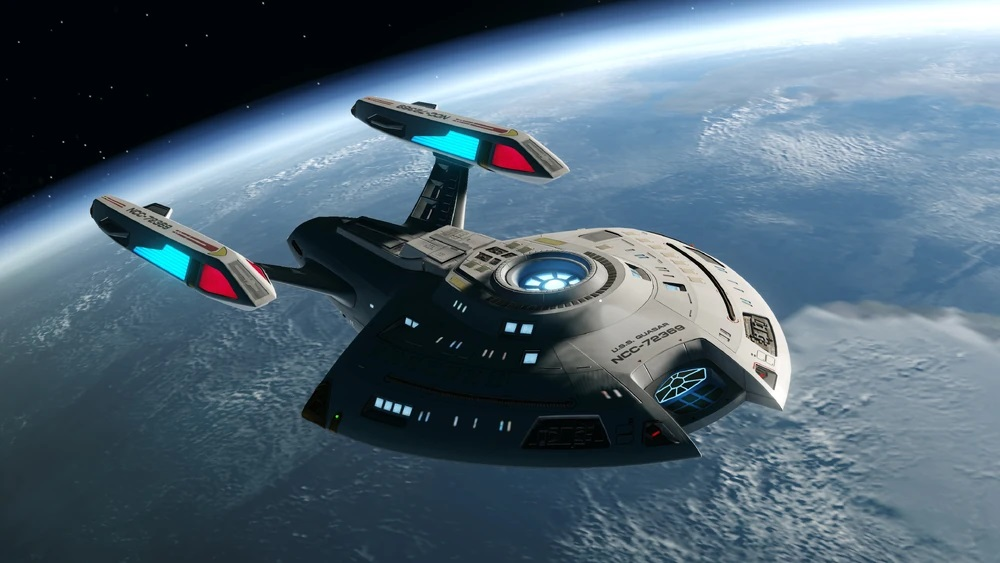
\includegraphics[width=1\linewidth]{img/RhodeIsland.jpg}
\end{figure*}



\chapter{Alleanza Ferengi-Romulana}
\begin{DndReadAloud}
Diario di Bordo del Comandante Tr'Ellor - RRW Thalassar

I sistemi di occultamento funzionano perfettamente. Né la Federazione né i nostri stessi... "alleati" a bordo sospettano i miei veri ordini.

Dodici giorni fa, il Pretore mi ha comandato di recuperare i sopravvissuti ferengi dalla nave danneggiata Profitto Dorato. Un'alleanza con dei mercanti... una macchia sull'onore romulano, ma necessaria. I ferengi possiedono dati cruciali sull'artefatto iconiano: coordinate, sequenze di attivazione, analisi energetiche. 

Informazioni che serviranno all'Impero.

Il DaiMon Brek si è dimostrato meno intollerabile del previsto. La sua avidità è prevedibile, ma la sua astuzia è... rispettabile. Vede "opportunità commerciali" dove noi vediamo vantaggio strategico militare. Parla di "rotte commerciali rivoluzionarie" mentre io contemplo il controllo dell'intero quadrante.

I sensori hanno confermato la presenza di altre navi dirette a Tartarus: la USS Venture della Federazione, una nave mineraria e una nave militare coloniale ignota.

I ferengi hanno già tentato due volte di violare i nostri database. Li lascio provare - rivela le loro priorità. Per ora, questa "collaborazione" serve allo scopo dell'Impero. Quando l'artefatto sarà nostro, rivaluterò l'utilità di questa alleanza.

Arrivo previsto tra 9 ore. Che gli antichi Iconiani siano scomparsi è irrilevante - la loro tecnologia presto servirà l'Impero Stellare Romulano.
    

\end{DndReadAloud}

\section{Background}
L'RRW Thalassar rappresenta una fragile alleanza tra Romulani e Ferengi, uniti da interessi diversi ma temporaneamente convergenti. I Romulani cercano un vantaggio strategico militare attraverso la tecnologia iconiana, mentre i Ferengi vedono potenziali profitti incalcolabili. Il Comandante Tr'Ellor, al comando della nave, mantiene un sottile equilibrio tra gli obiettivi dichiarati della missione e gli ordini segreti ricevuti dal Pretore romulano.
\section{Approccio Generale}

\begin{itemize}
    \item \textbf{Tensione costante}: Enfatizza il continuo tira e molla tra la strategia a lungo termine romulana e l'opportunismo ferengi
    \item \textbf{Duplicità come risorsa}: Questa nave può letteralmente "giocare su due tavoli" con il suo dispositivo di occultamento
    \item \textbf{Bilanciamento di QDP}: Concentrare gli sforzi su QDP Beta (tecnologia, potere, comunicazione)
    \item \textbf{Doppio gioco strategico}: Presentati come potenziale alleato a tutte le altre navi, ma mantieni sempre un'agenda nascosta
\end{itemize}

\section{Elementi Unici della Nave}

\begin{itemize}
    \item \textbf{Dispositivo di occultamento}: Permette alla nave di osservare non osservata e di ricomparire strategicamente
    \item \textbf{Dualità culturale}: Sfrutta la tensione tra la disciplina militare romulana e l'astuzia commerciale ferengi
    \item \textbf{Sindrome da assedio}: Tutti diffidano della RRW Thalassar (con buona ragione)
    \item \textbf{Tecnologia di singolarità quantica}: Speciale affinità per rilevare anomalie subspaziali
\end{itemize}

\section{Fasi dell'Avventura}
\subsection{Fase 1: Introduzione (15 minuti)
}

\begin{itemize}
    \item \textbf{Ambiente}: I romulani occupano la plancia principale, i ferengi hanno riservato i laboratori scientifici e le sezioni commerciali
    \item \textbf{Briefing iniziale}: Presenta il diario del Comandante Tr'Ellor che illustra la tensione interna
    \item \textbf{Presentazione PG}: Enfatizza quali personaggi sono romulani, quali ferengi, e se vi sono "infiltrati"
    \item \textbf{Definizione interessi}: Chiedi esplicitamente ai giocatori se stanno agendo nell'interesse romulano o ferengi
\end{itemize}

\subsection{Fase 2: Missioni Iniziali (60 minuti)}

\begin{itemize}
    \item Missione principale: "Recupero preventivo" - Un drone precedentemente inviato ha raccolto un frammento dell'artefatto iconiano
    \item \textbf{Complicazione}: Il recupero ha attivato un protocollo di sicurezza che minaccia la nave
    \item \textbf{Opportunità di QDP}:
    \begin{itemize}
    \item \textbf{Analisi del frammento}: +2 QDP Beta
    \item \textbf{Attivazione dell'occultamento in tempo}: +1 QDP Beta
    \item \textbf{Decodifica parziale dei segnali iconiani}: +2 QDP Alpha
    \end{itemize}
    \item \textbf{Comunicazioni}: Negli ultimi 10 minuti, stabilire comunicazioni con altre navi mantenendo una facciata amichevole
\end{itemize}

\subsection{Fase 3: Svolta (90 minuti)}

Attivazione anomalia: L'artefatto reagisce specificamente alla tecnologia di occultamento romulana
Manifestazioni iconiane:

La Risonanza dell'Occultamento: Il dispositivo crea microscopiche "bolle temporali" attorno alla nave
Il Paradosso del Profitto: Visioni contradditorie di possibili futuri per romulani e ferengi


Dilemma tattico: Rivelare informazioni cruciali alle altre navi per prevenire un disastro o usare la crisi come opportunità
Generazione QDP:

Calibrazione occultamento con frequenze iconiane: +3 QDP Beta
Manipolazione strategica delle altre fazioni: +2 QDP Beta



Fase 4: Conclusione (75 minuti)

Opzioni strategiche:

Acquisizione completa: Tentare di assumere il controllo esclusivo dell'artefatto (9 QDP Beta)
Alleanza strategica: Formare un'alleanza temporanea con una delle altre navi (5 QDP Beta + 2 QDP Alpha)
Duplicità massima: Fingere collaborazione mentre si sabotano gli sforzi delle altre navi (7 QDP Beta + infiltrazione)


Dinamiche di potere: Sfruttare divisioni tra le altre navi, specialmente tra la Federazione e la nave militare
Tiro di convergenza: Bonus +2 se in occultamento durante la fase critica

Meccaniche Speciali
Dispositivo di Occultamento

Attivazione: Costo 2 QDP Beta
Vantaggio principale: Impossibilità di essere rilevati dalle altre navi
Limitazioni: Comunicazioni e teletrasporto limitati mentre attivo
Disattivazione: Permette un elemento sorpresa strategico se usato nel momento giusto

Infiltrazione Mascherata

Costo: 3 QDP Beta
Effetto: Teletrasporto più difficile da rilevare verso altre navi
Utilizzo: Perfetto per il sabotaggio o il furto di informazioni

Suggerimenti per il Master

Chiedi regolarmente "State agendo nell'interesse romulano o ferengi?" per mantenere la tensione interna
Usa il comandante Tr'Ellor (NPC) come voce dell'Impero quando i giocatori pendono troppo verso gli interessi ferengi
Utilizza il DaiMon Brek (NPC) quando è necessario ricordare le opportunità commerciali
La paranoia è utile: dai ai giocatori l'impressione che tutte le altre navi stiano tramando contro di loro
L'occultamento è la vostra risorsa principale - usalo sia come vantaggio tattico che come occasione narrativa

QDP e Utilizzo

QDP Alpha: Comprensione, analisi (priorità secondaria)
QDP Beta: Tecnologia, comunicazione, potere (priorità primaria)
QDP Gamma: Raramente utile per questa nave, meglio scambiarlo con altre fazioni

Momenti Drammatici Chiave

Prima attivazione dell'occultamento
Decisione se rivelare la propria presenza alla Federazione
Momento in cui l'artefatto reagisce alla tecnologia romulana
Scelta finale: dominare, allearsi o sabotare

Interazioni con le Altre Navi

USS Venture (Federazione): Potenziale fonte di informazioni scientifiche, diffidente ma diplomatica
SS Halcyon (Mineraria): Alleati pragmatici, sfruttabili per le loro conoscenze sui minerali
HSS Ironclad (Militare): I più sospettosi, ma potenzialmente manipolabili se si fa leva sui loro timori

Ricorda: il vostro vantaggio principale è poter essere "ovunque e da nessuna parte" grazie all'occultamento, e poter giocare sia la carta della minaccia militare romulana che quella dell'opportunità commerciale ferengi!

Una fragile alleanza tra Ferengi e Romulani li ha portati nel sistema Tartarus. I Ferengi cercano profitto dall'artefatto, mentre i Romulani vogliono assicurarsi un vantaggio strategico. La tensione interna tra le due fazioni rappresenta una sfida costante.

\section{Background}

\section {Indicazioni per il master}

\subsection{Approccio Generale}

\begin{itemize}
    \item Enfatizza la tensione costante tra Romulani e Ferengi: un'alleanza necessaria ma scomoda
    \item Alterna momenti di effettiva collaborazione a momenti di sospetto reciproco
    \item Gioca sulla dualità di questa fazione: i Romulani sono calcolatori e strategici, i Ferengi opportunisti e pragmatici
    \item 
\end{itemize}
\subsection{Meccaniche dei QDP}

\begin{itemize}
    \item Concentrati principalmente sui QDP Beta (tecnologia, potere)
    \item Introduci situazioni in cui i Ferengi e i Romulani potrebbero avere preferenze divergenti su come utilizzare i QDP
    \item Incoraggia l'acquisizione opportunistica: intercettazione di comunicazioni, sottrazione di dati da altre fazioni
\end{itemize}

\subsection{Dinamiche Interne}

\begin{itemize}
    \item Crea occasionali "controlli di lealtà": chi è veramente al comando della missione?
    \item Quando i giocatori prendono decisioni importanti, chiedi loro se stanno agendo nell'interesse romulano o ferengi
    \item Utilizza la tensione interna come risorsa narrativa: "Il DaiMon Brek sembra particolarmente interessato a questa scoperta, il che fa sospettare il Centurione Verat"
\end{itemize}

\subsubsection{Interazioni con Altre Fazioni}

\begin{itemize}
    \item Incoraggia un approccio duplice: apparente cooperazione ma con agende nascoste
    \item Consenti ai giocatori di condividere informazioni deliberatamente imprecise o incomplete
    \item Offri opportunità per accordi segreti con singoli membri di altre fazioni
\end{itemize}

\subsection{Sfide Uniche}

\begin{itemize}
    \item Introduci occasionali problemi con il dispositivo di occultamento che potrebbero rivelare la loro posizione
    \item Crea situazioni in cui i Ferengi e i Romulani devono decidere quanto fidarsi l'uno dell'altro
    \item Presenta dilemmi dove la soluzione romulana (militare/strategica) e quella ferengi (commerciale/opportunistica) sarebbero radicalmente diverse
\end{itemize}

\subsection{Momenti Drammatici}

\begin{itemize}
    \item In fasi cruciali, ricorda ai giocatori ciò che è veramente in gioco per ciascuna cultura
    \item Per i Romulani: vantaggio strategico, superiorità militare, gloria dell'Impero
    \item Per i Ferengi: opportunità di profitto senza precedenti, accesso a mercati inediti
 
\end{itemize}
\subsection{Suggerimenti Narrativi}

\begin{itemize}
    \item "I vostri scanner rilevano un componente dell'artefatto particolarmente ricettivo alla vostra nave... i Ferengi pensano al profitto, i Romulani a un'arma."
    \item "Una comunicazione criptata dall'Impero richiede un aggiornamento sulla missione. Quanto rivelerete della vostra collaborazione con i Ferengi?"
    \item "Il DaiMon Brek propone un piano audace che potrebbe generare molti QDP, ma espone la nave a rilevamento."

\end{itemize}

\subsection{Gestione della Dualità}

\begin{itemize}
    \item Mantieni equilibrati i ruoli romulani e ferengi, evitando che una cultura domini completamente la narrazione
    \item Puoi usare NPC prominenti (il Comandante Tr'Ellor e il DaiMon Brek) per reindirizzare l'equipaggio se si allontana troppo dagli interessi di una delle due culture
    \item Occasionalmente, offri vantaggi esclusivi per azioni "tipicamente romulane" o "tipicamente ferengi"

\end{itemize}


\subsection {Informazioni}
\section{Il gioco}
\subsection{Introduzione}
\subsubsection{Brief}
Un drone inviato dai Ferengi ha raccolto un frammento dell'artefatto iconiano, ma il suo recupero ha attivato un protocollo di sicurezza alieno. La nave deve affrontare questa minaccia e negoziare con altre fazioni per mantenere il controllo del frammento.
\subsection{Missioni iniziali}
\subsection{Svolta}
\subsection{Conclusione}


\begin{landscape}

\begin{table}[htbp]
\centering
\caption{Scenari Possibili basati sui Punti Dati Quantici (QDP) e Relativi Effetti}
\small
\begin{tabular}{|p{2.3cm}|p{4cm}|p{4cm}|p{4cm}|p{4cm}|}
\hline
\textbf{Nave} & \textbf{Scenario Ottimale} & \textbf{Scenario Semi-Ottimale} & \textbf{Scenario Negativo} & \textbf{Catastrofe} \\ 
\hline
\textbf{USS Venture} & 

& 

& 

& 

\\ 
\hline
\textbf{RRW Thalassar} & 
\textbf{Vantaggio Strategico}

$>10$ Alpha, $<10$ Beta, $>10$ Gamma

\textit{Effetto}: I Romulani ottengono accesso controllato alla tecnologia dei portali, fornendo un vantaggio strategico mentre i Ferengi assicurano diritti commerciali esclusivi.
& 
\textbf{Attivazione Parziale}

?? Alpha, $<10$ Beta, $>10$ Gamma

\textit{Effetto}: Si ottiene una funzionalità limitata dei portali, offrendo alcuni vantaggi ma non un controllo completo. Nuove rotte commerciali si aprono.
& 
\textbf{Stallo Tecnologico}

?? Alpha, $>10$ Beta, ?? Gamma

\textit{Effetto}: L'artefatto viene messo in sicurezza ma produce poca tecnologia utilizzabile, frustrando sia gli obiettivi romulani che ferengi.
& 

\\ 
\hline
\textbf{SS Halcyon} & 

& 

& 

& 

\\ 
\hline
\textbf{HSS Ironclad} & 

& 

& 

& 

\\ 
\hline
\multicolumn{5}{|p{18.3cm}|}{} \\
\hline
\end{tabular}
\end{table}
\end{landscape}


\subsection{Indicazioni per il Master}
Ricorda ai giocatori la loro abilità unica di manipolazione e negoziazione
Possono tentare di influenzare il risultato finale giocando le altre fazioni l'una contro l'altra
La loro strategia di "doppio gioco" può essere rischiosa ma potenzialmente molto redditizia






\chapter{Mercantile}
\begin{DndReadAloud}    
Registro del Capitano Eliza Voss, SS Halcyon, Giorno 184 dalla partenza da Europa Nova

La missione procede secondo i parametri. Le scansioni preliminari del sistema Tartarus mostrano promettenti depositi di dilitio nel secondo asteroide del sistema, con tracce di tierillium che potrebbero giustificare l'installazione di una base estrattiva permanente. Il contratto con la Europa Nova Mining Consortium è chiaro: identificare, valutare, estrarre campioni. Semplice e redditizio.

Aspetta. Tian ha appena segnalato qualcosa di anomalo. I sensori hanno rilevato un'emissione energetica insolita dal quarto pianeta. Non corrisponde ad alcun profilo minerale nei nostri database.

\textit{Pausa nella registrazione}

Ho esaminato personalmente i dati. Questo non è un deposito minerario standard. L'emissione energetica è... pulsante. Ritmicamente, quasi come se stesse trasmettendo. E ci sono tracce di una lega cristallina con una composizione molecolare che sfida le leggi della fisica convenzionale. Dobbiamo investigare più a fondo.

Ho modificato la nostra rotta per portarci in orbita attorno al quarto pianeta. Stiamo rilevando anche interferenze nelle comunicazioni. Il nostro ultimo messaggio a Europa Nova è stato trasmesso con difficoltà, e la risposta è arrivata parzialmente corrotta.

\end{DndReadAloud}
\section {Indicazioni per il master}
\subsection{Atmosfera e tono}
Gestisci la SS Halcyon come una nave industriale fatiscente dove niente funziona al 100\%, tutto ha un suono inquietante, e l'equipaggio è costantemente in bilico tra terrore cosmico e necessità di sopravvivenza. L'artefatto iconiano rappresenta una minaccia esistenziale, ma anche l'unica speranza per la colonia di Europa Nova.

\subsection {Informazioni}
La SS Halcyon è una nave mineraria indipendente della colonia di Europa Nova. Il tuo equipaggio rappresenta un gruppo pragmatico di minatori, scienziati e tecnici interessati sia al potenziale economico dell'artefatto iconiano sia alla protezione della loro colonia dai suoi potenziali pericoli.

\section{Il gioco}
\subsection{Introduzione}
\subsubsection{Obiettivi della Fase}

\begin{itemize}
    \item Presentare la situazione e l'equipaggio
    \item Comunicare la missione iniziale
    \item Stabilire le prime strategie
\end{itemize}

\subsubsection{Azioni Suggerite}

\begin{enumerate}
    \item \textbf{Briefing iniziale}: Leggi il diario del Capitano Holloway per stabilire il tono della missione e la scoperta dell'anomalia nel sistema Tartarus.
    \item \textbf{Presentazione dell'equipaggio}: Chiedi a ciascun giocatore di presentare brevemente il proprio personaggio, focalizzandosi su competenze e motivazioni.
    \item \textbf{Situazione attuale}: Spiega che la SS Halcyon è già in orbita quando le altre navi iniziano ad arrivare. Sono i primi ad aver rilevato l'anomalia durante una spedizione di ricognizione mineraria.
    \item \textbf{Discussione iniziale}: Permetti ai giocatori di discutere brevemente approcci potenziali all'anomalia, enfatizzando i loro interessi primari:
     \begin{itemize}
     \item Valutazione del potenziale estrattivo
     \item Preoccupazioni per la sicurezza di Europa Nova
     \item Posizionamento rispetto alle grandi potenze in arrivo
     \end{itemize}
\end{enumerate}

\subsubsection{Nota al Master}
Sottolinea che mentre la loro nave ha capacità scientifiche e di estrazione superiori, è in svantaggio militare rispetto alle altre navi in arrivo. Il loro vantaggio sta nell'essere già presenti e nella conoscenza specialistica di geologia e estrazione.
\subsection{Missioni iniziali}


\subsubsection{Incidente Iniziale: "La Contaminazione Minerale"}


\begin{enumerate}
\item Situazione: Un container di campioni minerari nella stiva si apre improvvisamente. I minerali al suo interno pulsano con una luce aliena e cominciano a riconfigurare molecolarmente il metallo circostante.
\item Escalation: La contaminazione si diffonde rapidamente, fondendo strumenti e penetrando nei condotti dell'aria.
\item Complicazione horror:

\begin{itemize}
    \item Un tecnico di manutenzione nella stiva smette di rispondere
\item Le telecamere mostrano brevemente una figura distorta che sembra fusa con formazioni cristalline
\item I sistemi di comunicazione trasmettono solo sussurri incomprensibili e suoni di raschiamento
\end{itemize}

    \item Missione: L'equipaggio deve:

\begin{itemize}
    \item Isolare la contaminazione
    \item Recuperare o eliminare il tecnico (potenzialmente infetto)
    \item Contenere i campioni in camere di isolamento speciali
\end{itemize}

\end{enumerate}

\subsubsection{Check e Tiri Salvezza}

\begin{itemize}
    \item Tiro Salvezza Paura quando vedono il tecnico fuso con i cristalli
    \item Tiro Salvezza Corpo per chi entra nell'area contaminata senza protezione
    \item Aumento dello Stress per decisioni difficili (abbandonare il tecnico, distruggere campioni preziosi)
\end{itemize}

\subsubsection{Frammenti di Informazione (da recuperare durante la missione)}

\begin{itemize}
    \item Dati scientifici che suggeriscono che l'artefatto "comunica" attraverso riconfigurazione minerale
    \item Registrazioni del tecnico che parlava di "voci dalle rocce" giorni prima dell'incidente
    \item Scansioni che mostrano che i minerali stanno creando una rappresentazione in miniatura dell'artefatto
    \item 
\end{itemize}
\subsubsection{Comunicazioni con Altre Navi (ultimi 10 minuti)}

\begin{itemize}
    \item La Federazione offre assistenza medica, ma vuole accesso ai vostri dati
    \item I sensori rilevano brevi flash di occultamento vicino alla nave
    \item La nave militare della Coalizione mantiene una "distanza di sicurezza", considerandovi potenzialmente contaminati
\end{itemize}

\subsubsection{Generazione di QDP (derivante dal terrore)}

\begin{itemize}
    \item Contenimento della contaminazione: +2 QDP Gamma
    \item Analisi dei campioni mutati: +1 QDP Alpha
    \item Sacrificio personale per recuperare dati cruciali: +2 QDP di tipo variabile
\end{itemize}

\subsection{Svolta}

\subsubsection{Obiettivi della Fase}

Affrontare l'intensificazione dell'anomalia e l'attivazione parziale del portale
Collaborare con altri tavoli per decifrare i segnali iconiani
Gestire una crescente minaccia per Europa Nova

\subsubsection{Situazione Critica}

\begin{enumerate}
    \item L'intensificazione: L'anomalia inizia a pulsare più intensamente, creando onde subspaziali che interferiscono con i sistemi della nave.
    \item La minaccia: Il portale inizia ad attivarsi parzialmente, creando una connessione instabile con lo spazio vicino a Europa Nova - il pianeta della colonia è direttamente minacciato!
    \item Manifestazioni iconiane:

\begin{itemize}
    \item Proiezioni Cartografiche: Mappe stellari appaiono spontaneamente, mostrando connessioni tra sistemi stellari
    \item Cristallizzazioni Spontanee: Formazioni cristalline crescono rapidamente nella stiva di carico
    \item Alterazioni Energetiche: I sistemi energetici oscillano seguendo pattern specifici
\end{itemize}

\end{enumerate}

\subsubsection{Cooperazione Necessaria}

Stabilire comunicazioni con le altre navi diventa essenziale
Ogni nave possiede un pezzo del puzzle necessario per prevenire un disastro
L'equipaggio deve decidere quanto rivelare delle proprie scoperte

\subsubsection{Generazione di QDP}

Analisi delle proiezioni cartografiche: +2 QDP Alpha
Stabilizzazione dei sistemi durante l'intensificazione: +2 QDP Gamma
Partecipazione agli enigmi collaborativi: +3 QDP (mix di tipi)
Condivisione strategica di informazioni con altre fazioni: +1-2 QDP Beta



\subsection{Conclusione}
\subsubsection{Obiettivi della Fase}

Contribuire alla decisione finale sul destino del portale
Formare alleanze o affrontare conflitti con le altre navi
Proteggere gli interessi di Europa Nova e dell'equipaggio

\subsubsection{Opzioni Strategiche}
L'equipaggio deve posizionarsi rispetto a tre possibili approcci all'artefatto:

\begin{enumerate}
    \item Stabilizzazione:
    \begin{itemize}
        
    \item Utilizzare le conoscenze geologiche per creare un "ancoraggio minerale" che stabilizzi il portale
    \item Costo: 5 QDP Gamma + 3 QDP Alpha
    \item Risultato: Il portale rimane dormiente ma intatto per studi futuri
    
    \end{itemize} 
    \item Distruzione:
    \begin{itemize}
        
    
    \item Sfruttare l'esperienza in demolizioni per identificare punti deboli nell'artefatto
    \item Costo: 6 QDP Gamma + 2 QDP Beta
    \item Risultato: Il portale viene disattivato permanentemente, eliminando rischi e opportunità
    \end{itemize}
    
    \item Attivazione Controllata:
    \begin{itemize}
    
    \item Utilizzare il "traduttore minerale" per stabilire un controllo limitato sul portale
    \item Costo: 4 QDP di ogni tipo
    \item Risultato: Il portale diventa operativo ma con limitazioni di sicurezza
    \end{itemize}
\end{enumerate}

\subsubsection{Dinamiche di Potere}

\begin{itemize}
    \item La nave della Federazione probabilmente spingerà per la stabilizzazione o un'attivazione controllata
    \item I Romulani cercheranno il controllo completo della tecnologia
    \item La nave militare della Coalizione potrebbe preferire la distruzione per eliminare la minaccia
\end{itemize}

\subsubsection{Tiro di Convergenza}
Durante il confronto finale, l'equipaggio della Halcyon riceve:

\begin{itemize}
    \item Bonus di +1 per ogni QDP Gamma speso
    \item Bonus aggiuntivo di +2 se utilizzano la loro conoscenza mineralogica in modo creativo
    \item Malus di -1 se sono in conflitto diretto con una nave militare
\end{itemize}

\subsection{Epilogo}

\begin{itemize}
    \item Descrivi come la risoluzione impatta Europa Nova e il futuro dell'equipaggio
    \item Concentrati sulle conseguenze economiche e di sicurezza per la colonia mineraria
    \item Offri a ciascun giocatore l'opportunità di descrivere brevemente il destino del proprio personaggio
\end{itemize}




\section{Riferimenti rapidi}
\subsection{Personaggi Chiave}

\begin{itemize}
    \item \textbf{Capitano Mira Holloway}: Pragmatica, terza generazione di minatori
    \item \textbf{Marcus Chen}: Ex-ufficiale della Flotta, esperto di ingegneria
    \item \textbf{Dottoressa Eliza Novak}: Geologa specializzata, adattata geneticamente
    \item \textbf{Soren Volkov}: Sicurezza, ex-mercenario con sangue betazoide
    \item \textbf{Altri membri dell'equipaggio}: Vedere schede personaggio
    \item 
\end{itemize}
\subsection{QDP e Utilizzo}
\begin{itemize}
    \item \textbf{QDP Alpha}: Analisi, comprensione, stabilizzazione
    \item \textbf{QDP Beta}: Comunicazione, influenza, tecnologia
    \item \textbf{QDP Gamma}: Risorse, materiali, estrazione
\end{itemize}

\subsection{Capacità Uniche della Nave}

\begin{itemize}
    \item Sistemi di estrazione mineraria avanzati
    \item Scanner geologici superiori a quelli standard
    \item Esperienza con materiali esotici e pericolosi
    \item Moduli di contenimento per materiali instabili
\end{itemize}

\subsection{Meccaniche di Teletrasporto in presenza di Interferenze Iconiane}

\begin{itemize}
    \item \textbf{Costo base}: 3 QDP per attivare un singolo teletrasporto
    \item \textbf{Bonus minerario}: +1 ai tiri di teletrasporto quando coinvolgono materiali/minerali
    \item \textbf{Capacità unica}: "Estrazione di Emergenza" - Può recuperare personale in pericolo (4 QDP)
    \item \textbf{Rischi}: Maggiori in presenza di minerali attivi o in risonanza con l'artefatto
\end{itemize}


\section {Consigli}
\begin{itemize}
    \item Enfatizza l'approccio pragmatico e indipendente dell'equipaggio
    \item Ricorda che l'equipaggio è esperto nell'improvvisare soluzioni con risorse limitate
    \item Usa le manifestazioni iconiane legate ai minerali per creare momenti di meraviglia
    \item Sfrutta la tensione tra il potenziale profitto dell'artefatto e il rischio per la colonia
    \item Incoraggia i giocatori a usare la loro conoscenza specialistica come merce di scambio nelle negoziazioni
    \item Durante la Fase 3, crea un senso di urgenza genuino quando Europa Nova viene minacciata
\end{itemize}


\chapter{Militari}
\begin{DndReadAloud}
Registro di comando, capitano Darius Reed, HSS Ironclad, 22° ciclo, Anno di Fondazione 87
    
Alto Comando, questo è il Comandante Reed. La missione procede come ordinato. La Ironclad è in rotta verso il sistema Tartarus dopo aver intercettato comunicazioni criptate dalla Federazione riguardanti un'anomalia di interesse strategico.

L'intelligence della Coalizione ha identificato attività insolita in quel settore. Prima una nave mineraria indipendente, la SS Halcyon, ha deviato improvvisamente dalla sua rotta dichiarata. Poi, trasmissioni subspaziali frammentarie hanno menzionato "tecnologia antica" e "potenziale rischio". Infine, abbiamo confermato che una nave della Federazione classe Galaxy, la USS Venture, è stata inviata con priorità massima.

Qualunque cosa abbiano trovato, è abbastanza importante da far correre la Federazione. E se è importante per loro, è importante per la sicurezza della Coalizione delle Colonie Indipendenti.

Il nostro analista tattico, Maggiore Chen, ha confrontato le firme energetiche intercettate con il nostro database. C'è una corrispondenza parziale con registrazioni frammentarie di tecnologia iconiana. Se confermato, questo rappresenta sia un'opportunità che una minaccia esistenziale per le nostre colonie.

I membri del Consiglio sanno bene quanto le nostre colonie siano vulnerabili, strette tra Federazione, Klingon e interessi Romulani. La nostra indipendenza si basa esclusivamente sulla nostra capacità di difenderci. Una tecnologia che permette il trasporto istantaneo attraverso la galassia cambierebbe radicalmente l'equilibrio di potere.

I miei ordini sono chiari: valutare la minaccia, acquisire qualsiasi tecnologia difensiva possibile, e se necessario, neutralizzare la situazione piuttosto che permettere che cada nelle mani sbagliate. E sì, per quanto riguarda la Coalizione, sia la Federazione che i Romulani costituiscono "mani sbagliate".

La Ironclad non è una nave scientifica. È un incrociatore pesante con equipaggio militare. Non siamo attrezzati per ricerca approfondita, ma i nostri specialisti di armi e difesa sono i migliori della Coalizione. Se qualcuno può identificare le applicazioni difensive di questa tecnologia, siamo noi.

I sensori rilevano già attività nel sistema Tartarus. La nave mineraria è in orbita attorno al quarto pianeta. La nave della Federazione arriverà entro poche ore. E c'è qualcos'altro... brevi apparizioni sui sensori che suggeriscono una nave occultata. Probabilmente Romulana.

Ho attivato i protocolli di guerra elettronica e messo gli armamenti in stato di prontezza. La nostra posizione diplomatica rimane neutra fino a quando non valutiamo la situazione, ma non saremo colti impreparati.

Il Maggiore Chen suggerisce che potremmo usare la nostra conoscenza più approfondita della regione della Shackleton Expanse come vantaggio negoziale. Concordo. La Federazione ha studiato l'area solo superficialmente, e i Romulani si affidano principalmente allo spionaggio. Il nostro tempo in questi settori periferici ci ha dato una comprensione che le maggiori potenze non possiedono.

Mentre ci avviciniamo, ho ordinato scansioni a spettro completo. Se questo è davvero un artefatto iconiano, dobbiamo determinare se rappresenta una minaccia immediata per le nostre colonie. La storia ci ha insegnato che tecnologie aliene incomprensibili raramente portano benefici senza conseguenze.

Una cosa è certa: non permetterò che questa tecnologia venga usata contro il nostro popolo. Se non possiamo controllarla, dobbiamo assicurarci che nessun altro possa farlo.
Arrivo previsto al sistema Tartarus in 4 ore. La Ironclad è pronta.

\end{DndReadAloud}
\section {Indicazioni per il master}

Nave Militare della Coalizione - Sistema Diceless

"Non siamo qui per esplorare. Non siamo qui per profitto. Siamo qui per proteggere. Se questa reliquia iconiana minaccia i nostri mondi, è nostro dovere neutralizzarla. Se altre potenze intendono sfruttarla, è nostro dovere impedirlo. La Coalizione si è formata perché le grandi potenze non si preoccupano dei piccoli. Oggi dimostriamo che i piccoli hanno denti."
— Comandante Aleksander Novak, briefing pre-missione

\subsection{FILOSOFIA DI GIOCO DICELESS}
Gestisci la HSS Ironclad con un approccio narrativo basato su:

\begin{itemize}
    \item Competenza dei personaggi: I membri dell'equipaggio sono professionisti altamente addestrati
    \item Risoluzioni basate su narrazione: Le azioni riescono o falliscono in base alla logica narrativa, non ai dadi
    \item Competenze come autorizzazioni: Se un personaggio ha una competenza, può eseguire azioni in quell'ambito
    \item Tensione creata da scelte difficili, non da fallimenti casuali
\end{itemize}

\subsection{FASE 1: INTRODUZIONE (15 minuti)}
\subsubsection{Ambientazione della Scena}

La nave è pulita, efficiente ma austera - risorse limitate usate con massima efficienza
L'equipaggio è disciplinato ma non rigido, unito da lealtà reciproca più che da gerarchia
I display mostrano costantemente scansioni dell'anomalia e delle altre navi in avvicinamento

\subsubsection{Briefing Iniziale}
Leggi con tono determinato e cauto:
"Equipaggio della Ironclad, siamo qui con una missione chiara. L'anomalia rilevata nel sistema Tartarus presenta firme energetiche coerenti con tecnologia iconiana. Analisi preliminari indicano potenziale attivazione di un nodo di portale. Se il portale si attivasse incontrollato, potrebbe aprire varchi verso qualsiasi mondo, inclusi quelli della Coalizione. Non possiamo permetterlo. Non siamo soli. La Federazione ha inviato la USS Venture, classe Nova. Una nave mineraria, la SS Halcyon, è già in orbita. E i nostri sensori rilevano tracce di una nave occultata - presumibilmente romulana. Ricordate: protezione, non provocazione. Ma se questa tecnologia deve essere neutralizzata, lo faremo senza esitazione."
\subsubsection{Presentazione Personaggi}

Chiedi ai giocatori di descrivere il loro personaggio con enfasi su:

\begin{itemize}
    \item La loro specializzazione e come supporta la missione
    \item Un aspetto della loro identità culturale (umano caldosiano, Veshi, Tellarite, rifugiato romulano, etc.)
    \item Una ragione personale per la quale proteggere la Coalizione è importante per loro
\end{itemize}



\subsubsection{Creazione di Tensione}

\begin{itemize}
    \item Illustra come la nave sia tecnologicamente inferiore alle altre potenziali minacce
    \item Sottolinea che l'equipaggio diversificato è la loro forza principale
    \item Chiedi ad ogni giocatore di esprimere una preoccupazione del proprio personaggio
\end{itemize}

\subsection{FASE 2: MISSIONI INIZIALI (60 minuti)}
\subsubsection{Missione Principale: "Perimetro di Sicurezza"}

\begin{enumerate}
    \item Situazione: La Ironclad deve stabilire un perimetro di sicurezza attorno all'anomalia senza provocare incidenti diplomatici.
    \item Complicazioni:
    \begin{itemize}
    \item I sensori rilevano brevi picchi energetici dall'anomalia che potrebbero essere tentativi di comunicazione
    \item La nave occultata (romulana) sembra manovrare per avvicinarsi all'anomalia
    \item La Federazione richiede coordinamento delle operazioni, implicando una subordinazione della Ironclad
    
    \end{itemize}
    \item Sfide per l'equipaggio:
    \begin{itemize}
    \item Stabilire un sistema di monitoraggio che mappi la zona senza apparire ostili
    \item Decidere come rispondere ai tentativi di avvicinamento romulani
    \item Mantenere indipendenza operativa senza alienare potenziali alleati
    \end{itemize}
    
    \item Manifestazione dell'Anomalia: Durante l'operazione, l'anomalia emette un impulso che causa una breve proiezione olografica sulla plancia - una mappa stellare con particolare enfasi sui mondi della Coalizione.
\end{enumerate}

\subsubsection{Risoluzione Narrativa}
Invece di tirare dadi, risolvi le situazioni basandoti su:

\begin{itemize}
    \item Competenza: Se un personaggio ha la competenza appropriata, riesce nell'azione base
    \item Complessità: Per azioni complesse, richiedi descrizioni dettagliate del loro approccio
    \item Conseguenze: Anche i successi hanno costi o complicazioni
    \item Collaborazione: Due personaggi che lavorano insieme possono superare sfide più difficili
\end{itemize}

\subsubsection{Frammenti di Informazione}
Durante questa fase, l'equipaggio scopre:

\begin{itemize}
    \item L'anomalia reagisce in modo inaspettato quando scansionata con determinate frequenze militari
    \item Il pattern dell'anomalia sembra contenere elementi di navigazione o targetizzazione
    \item Esistono similitudini tra alcuni protocolli difensivi della Coalizione e certi pattern dell'anomalia
\end{itemize}

\subsubsection{Prime Comunicazioni (ultimi 10 minuti)}

\begin{itemize}
    \item La USS Venture propone uno scambio di dati scientifici
    \item La nave mineraria Halcyon rivela una reazione anomala dei loro minerali all'artefatto
    \item Comunicazioni criptate suggeriscono che i Romulani stanno tentando di accedere all'artefatto
\end{itemize}

\subsubsection{Generazione di QDP}

\begin{itemize}
    \item Stabilimento efficace del perimetro di sicurezza: +2 QDP Beta
    \item Analisi della proiezione stellare: +1 QDP Alpha + 1 QDP Beta
    \item Gestione diplomatica delle altre navi: +2 QDP Beta
\end{itemize}

\subsection{FASE 3: SVOLTA (90 minuti)}
\subsubsection{La Crisi: "Segnale di Targetizzazione"}
L'anomalia iconiana si attiva parzialmente, emettendo un segnale che la Ironclad riconosce come simile a un sistema di targetizzazione militare. L'analisi rivela che l'artefatto sta "puntando" verso diversi mondi, incluse colonie della Coalizione.

\begin{enumerate}
    \item Escalation della minaccia:
    \begin{itemize}
    \item I sensori indicano che l'artefatto sta creando micro-portali instabili
    \item Uno di questi portali si apre brevemente, mostrando una colonia della Coalizione (Caldos II)
    \item L'analisi temporale indica un conto alla rovescia verso un'attivazione completa
    \end{itemize}
    \item Manifestazioni iconiane:
    \begin{itemize}
    \item Il Giuramento del Guerriero: I sistemi d'arma della nave iniziano a pulsare seguendo pattern specifici, come se l'artefatto stesse "testando" le capacità difensive della nave
    \item Le Voci dei Mondi Perduti: I membri dell'equipaggio più diversificati (Veshi telepatica, rifugiato romulano, umano geneticamente modificato) cominciano a ricevere visioni di mondi iconiani
    \end{itemize}
    \item Dilemma tattico:
    \begin{itemize}
    \item Una risposta aggressiva potrebbe accelerare l'attivazione dell'artefatto
    \item Un approccio passivo potrebbe permettere alle altre navi di prendere il controllo
    \item L'attivazione completa minaccia direttamente i mondi della Coalizione
    \end{itemize}
\end{enumerate}




\subsubsection{Risoluzione Narrativa in Situazioni di Crisi}

\begin{itemize}
    \item Per decisioni ad alta tensione, offri ai giocatori opzioni con conseguenze chiare
    \item Utilizza il principio di "sì, ma..." permettendo successi con complicazioni
    \item Per conflitti di priorità tra personaggi, incoraggia il dibattito in-character
\end{itemize}

\subsubsection{Generazione di QDP}
\begin{itemize}
    \item Analisi del sistema di targetizzazione: +2 QDP Alpha
    \item Stabilizzazione dei micro-portali: +2 QDP Beta
    \item Interpretazione delle visioni: +2 QDP Alpha
    \item Cooperazione con altre navi: +2 QDP Beta
\end{itemize}

\subsection{FASE 4: CONCLUSIONE (75 minuti)}
\subsubsection{La Scelta Finale}
L'equipaggio deve decidere il destino dell'artefatto mentre il conto alla rovescia verso l'attivazione completa prosegue. La tensione è massima - la sicurezza della Coalizione è in gioco.
\subsubsection{Opzioni Strategiche}
\begin{enumerate}
    \item \textbf{Neutralizzazione Completa}:
     \begin{itemize}
     \item Approccio: Utilizzare i sistemi d'arma della Ironclad per disabilitare l'artefatto
     \item Costo: 6 QDP Beta + 2 QDP Alpha
     \item Conseguenze: L'artefatto viene neutralizzato ma qualsiasi potenziale beneficio è perso, possibile conflitto con altre navi
    \item \end{itemize}
     
     
     \item \textbf{Scudo Difensivo}:
     
     \begin{itemize}
     \item Approccio: Creare una matrice di interferenza che blocchi selettivamente i portali verso i mondi della Coalizione
     \item Costo: 4 QDP Beta + 4 QDP Alpha
     \item Conseguenze: I mondi della Coalizione sono protetti, ma l'artefatto rimane attivo e accessibile ad altri
     \end{itemize}
     
     
    \item \textbf{Riconfigurazione Tattica}:
     
     \begin{itemize}
     \item Approccio: Utilizzare la comprensione dei sistemi militari iconiani per riprogrammare l'artefatto
     \item Costo: 5 QDP di ogni tipo
     \item Conseguenze: L'artefatto diventa un asset difensivo per la Coalizione, ma richiede monitoraggio costante
     \end{itemize}
\end{enumerate}



\subsubsection{Dinamiche di Potere e Diplomazia}

\begin{itemize}
    \item Le altre navi avranno obiettivi probabilmente incompatibili con quelli della Ironclad
    \item Possibilità di alleanze tattiche temporanee basate su interessi convergenti
    \item Opzioni per bluff e negoziazioni sotto pressione
\end{itemize}

\subsubsection{Risoluzione Narrativa del Confronto Finale}

\begin{itemize}
    \item Struttura la scena come una serie di mosse e contromosse diplomatiche e tattiche
    \item Utilizza un sistema di countdown visibile per creare urgenza
    \item Risolvi le azioni basandoti sulla qualità del piano, le risorse investite (QDP) e il posizionamento precedente
\end{itemize}

\subsection{Epilogo}

\begin{itemize}
    \item Descrivi come la risoluzione impatta l'equilibrio di potere nella Shackleton Expanse
    \item Esplora le conseguenze per i mondi della Coalizione
    \item Offri a ciascun giocatore l'opportunità di descrivere il futuro del proprio personaggio
\end{itemize}

\section{RISORSE DI RIFERIMENTO RAPIDO}
\subsection{Personaggi Chiave}

\begin{itemize}
    \item \textbf{Comandante Aleksander Novak}: Umano caldosiano, veterano pragmatico
    \item \textbf{Tenente Comandante Sadira Veshi}: Prima ufficiale anfibio-umanoide con capacità telepatiche limitate
    \item \textbf{Maggiore Kron}: Capo sicurezza tellarite, combattivo ma leale
    \item \textbf{Tenente Sovar}: Ufficiale scientifico romulano rifugiato, sotto costante sospetto
    \item Altri membri dell'equipaggio: Vedere schede personaggio
\end{itemize}

\subsection{QDP e Utilizzo}

\begin{itemize}
    \item \textbf{QDP Alpha}: Comprensione, analisi, conoscenza
    \item \textbf{QDP Beta}: Tattiche, diplomazia, sistemi difensivi
    \item \textbf{QDP Gamma}: Utilizzato raramente dalla Ironclad, principalmente per operazioni materiali
\end{itemize}

\subsection{Elementi Unici della Nave}

\begin{itemize}
    \item Equipaggio multiculturale con prospettive diverse sullo stesso problema
    \item Sistemi difensivi adattati da tecnologie di diverse culture
    \item Catena di comando flessibile basata sull'expertise più che sul grado
\end{itemize}

\subsection{Principi Narrativi per Risoluzioni Diceless}

\begin{itemize}
    \item Competenza come assunto base: L'equipaggio è capace nel proprio campo
    \item Scelte significative al posto di tiri casuali
    \item Conseguenze naturali invece di penalità arbitrarie
    \item Collaborazione e sinergia tra diverse specializzazioni
\end{itemize}


\begin{landscape}

\begin{table}[htbp]
\centering
\caption{Scenari Possibili basati sui Punti Dati Quantici (QDP) e Relativi Effetti}
\small
\begin{tabular}{|p{2.3cm}|p{4cm}|p{4cm}|p{4cm}|p{4cm}|}
\hline
\textbf{Nave} & \textbf{Scenario Ottimale} & \textbf{Scenario Semi-Ottimale} & \textbf{Scenario Negativo} & \textbf{Catastrofe} \\ 
\hline
\textbf{USS Venture} & 

& 

& 

& 

\\ 
\hline
\textbf{RRW Thalassar} & 

& 

& 

& 

\\ 
\hline
\textbf{SS Halcyon} & 

& 

& 

& 

\\ 
\hline
\textbf{HSS Ironclad} & 

& 
\textbf{Protocollo di Neutralizzazione}

$4$-$8$ Alpha, $4$-$8$ Beta, $4$-$8$ Gamma

\textit{Effetto}: L'artefatto viene neutralizzato con successo, impedendo a qualsiasi fazione di ottenere un vantaggio e mantenendo l'equilibrio di potere.
& 
\textbf{Contenimento Instabile}

$>8$ Alpha, $>8$ Beta, $>8$ Gamma

\textit{Effetto}: L'artefatto è parzialmente neutralizzato ma rimane una potenziale minaccia, richiedendo costante sorveglianza militare.
& 

\\ 
\hline
\multicolumn{5}{|p{18.3cm}|}{\textbf{Scenario Neutro - Spegnimento Completo}: La tecnologia viene completamente disattivata, mantenendo l'attuale equilibrio di potere. La HSS Ironclad (Militare) è particolarmente interessata a questo scenario, preferendolo ad altri potenziali risultati.} \\
\hline
\end{tabular}
\end{table}
\end{landscape}

\section{CONSIGLI PER IL MASTER}

\begin{itemize}
    \item Enfatizza la diversità culturale dell'equipaggio come fonte di forza e occasionalmente di tensione
    \item Usa la limitata potenza della nave come elemento di tensione narrativa
    \item Crea momenti per ciascun personaggio dove la loro cultura o background specifico fornisce una prospettiva unica
    \item Bilancia l'approccio militare con considerazioni diplomatiche ed etiche
    \item Ricorda che la missione primaria è proteggere la Coalizione, non necessariamente distruggere l'artefatto
    \item Crea situazioni dove i personaggi devono scegliere tra sicurezza immediata e benefici potenziali a lungo termine
\end{itemize}


\part{Appendice}


\chapter{Background}


\section {Ferengi}

\begin{figure}
    \centering
    
\includegraphics[width=1\linewidth]{img/Logo_Ferengi.svg.png}
\end{figure}
I Ferengi\footnote{\url{https://memory-alpha.fandom.com/wiki/Ferengi}} sono una specie umanoide originaria del pianeta Ferenginar, riconoscibili dalle caratteristiche orecchie larghe e lobate, dalla bassa statura, e dalla testa priva di capelli con una struttura cranica rugosa. La loro società è interamente organizzata attorno al profitto e al commercio, regolata dalle 285 Regole dell'Acquisizione.

\subsection{Cultura e Società}
La società ferengi è dominata dal commercio. Il più alto organo di governo è il Grande Nagus, che sovrintende all'Autorità Commerciale Ferengi. Il profitto non è solo un obiettivo economico, ma un vero e proprio imperativo morale e religioso. Lo status sociale è determinato esclusivamente dalla ricchezza e dall'abilità commerciale.

Fino a tempi recenti, le femmine ferengi non potevano indossare vestiti, guadagnare profitto o viaggiare, sebbene queste restrizioni siano state progressivamente allentate sotto l'influenza delle riforme del Grande Nagus Rom.

\subsection{Valori Fondamentali}
\begin{itemize}
    \item Il profitto è il valore supremo
    \item I contratti sono sacri (ma sempre soggetti a interpretazione)
    \item Ogni individuo è responsabile del proprio successo o fallimento
    \item L'inganno è accettabile se porta al profitto
    \item Le relazioni personali sono secondarie rispetto all'opportunità commerciale
\end{itemize}

\subsection{Tecnologia}
Nonostante la loro reputazione di avari, i Ferengi possiedono tecnologia avanzata, spesso acquisita attraverso scambi commerciali. Sono particolarmente abili nell'adattare e migliorare tecnologie aliene per i loro scopi.

Le loro navi, chiamate Marauder, hanno capacità di combattimento limitate rispetto a quelle della Flotta Stellare o dell'Impero Romulano, ma sono equipaggiate con avanzati sistemi di scansione e analisi, perfetti per identificare opportunità di profitto.

\subsection{Approccio Diplomatico}
I Ferengi sono tecnicamente neutrali nelle maggiori dispute politiche del quadrante. Commerciano con tutti, purché ci sia profitto da realizzare. Questa neutralità ha permesso loro di stabilire rapporti commerciali anche in periodi di conflitto tra le maggiori potenze.

Nelle negoziazioni, i Ferengi sono noti per:
\begin{itemize}
    \item Iniziare con richieste esorbitanti per poi "concedere" ciò che volevano davvero
    \item Nascondere clausole in contratti complessi
    \item Cercare sempre il vantaggio personale piuttosto che accordi equi
    \item Rispettare alla lettera (ma non nello spirito) gli accordi raggiunti
\end{itemize}

I Ferengi non sono intrinsecamente ostili o malvagi - semplicemente vedono l'universo attraverso la lente del potenziale profitto, una visione spesso incomprensibile alle culture che valorizzano obiettivi più astratti come esplorazione, onore o progresso scientifico.

\section {Romulani}
I Romulani sono una specie umanoide discendente da coloni vulcaniani che rifiutarono la filosofia della logica di Surak. Fisicamente simili ai Vulcaniani, si distinguono per le creste ossee frontali e un'espressività emotiva assente nei loro cugini vulcaniani. Originari del pianeta Romulus (distrutto nel 2387), sono una delle maggiori potenze del quadrante Beta.
\subsection{Cultura e Società}
\begin{figure}
    \centering
    
\includegraphics[width=1\linewidth]{img/jxvppos0w9941.png}
\end{figure}

La società romulana è edificata attorno a principi di segretezza, superiorità culturale e servizio allo stato. L'Impero Stellare Romulano è governato da un Senato con a capo un Pretore, affiancato dal potente servizio segreto Tal Shiar che mantiene il controllo interno. La cultura romulana valorizza fortemente l'onore personale, la lealtà alla famiglia e allo stato, e la capacità di manipolare eventi a proprio vantaggio.
La società è altamente stratificata, con una classe dirigente patrizia e una popolazione ordinaria che serve l'Impero. L'avanzamento sociale è possibile attraverso il servizio militare o successi politici significativi.
\subsection{Valori Fondamentali}

\begin{itemize}
    \item Superiorità dell'Impero Romulano
    \item Segretezza e discrezione in ogni azione
    \item Pazienza strategica e pianificazione a lungo termine
    \item Astuzia e inganno come strumenti legittimi di statecraft
    \item Lealtà alla famiglia e alla struttura di comando
\end{itemize}

\subsection{Tecnologia}
I Romulani possiedono tecnologia militare tra le più avanzate del quadrante, con due innovazioni distintive:

\begin{itemize}
    \item Dispositivo di occultamento, che rende le loro navi invisibili ai sensori convenzionali
    \item Motori ad energia basati su singolarità quantiche artificiali
\end{itemize}

Le loro navi da guerra, in particolare i Warbird classe D'deridex, sono potenti piattaforme militari progettate per operazioni a lungo raggio e azioni strategiche.

\subsection{Approccio Diplomatico}
I Romulani sono noti per:

\begin{itemize}
    \item Preferire l'osservazione prolungata prima dell'azione
    \item Creare alleanze temporanee basate su interessi convergenti
    \item Usare disinformazione e agenti infiltrati
    \item Evitare conflitti aperti quando possibile, preferendo manovre indirette
    \item Mantenere un'aura di mistero e imprevedibilità
\end{itemize}

Sebbene siano considerati antagonisti dalle potenze della Federazione, i Romulani non sono motivati da semplice malvagità, ma da un profondo senso di responsabilità verso la sopravvivenza e l'espansione dell'Impero. La loro filosofia pragmatica vede il resto della galassia come una potenziale minaccia da neutralizzare o una risorsa da utilizzare.
Le relazioni con le altre potenze sono caratterizzate da periodi alterni di ostilità aperta e diplomazia cauta, con un sottofondo costante di manovre di intelligence e posizionamento strategico.

L'avventura si svolge circa 40 anni dopo l'esplosione della stella Hobus.

Dopo la catastrofica esplosione della stella Hobus nel 2387, che causò la distruzione di Romulus e Remus, l'Impero Stellare Romulano ha subito una trasformazione drammatica e dolorosa.
\subsection{Diaspora e Frammentazione Politica
}
Con la distruzione del pianeta natale, milioni di romulani sono diventati rifugiati, dispersi in colonie periferiche e insediamenti d'emergenza. L'Impero, una volta monolitico, si è frammentato in diverse fazioni:

\begin{itemize}
    \item Il \textbf{Governo Imperiale Provvisorio}, che mantiene il controllo sulle colonie principali e sulla flotta centrale
    \item Lo \textbf{Stato Libero Romulano}, una fazione separatista con una visione più progressista
    \item Diverse \textbf{Casate Patrizie} che hanno stabilito domini quasi-indipendenti
    \item \textbf{Enclavi Militari} guidate da comandanti della flotta che operano con crescente autonomia
\end{itemize}

\subsection{Nuovi Centri di Potere}
In assenza di Romulus, diverse colonie hanno assunto maggiore importanza:

\begin{itemize}
    \item \textbf{Rator III} è diventato il principale centro amministrativo dell'Impero
    \item \textbf{Achernar Prime} ospita gran parte dell'industria militare romulana
    \item \textbf{Virinat} funge da importante centro agricolo per sostenere la popolazione
    \item \textbf{Crateris} è emersa come centro commerciale e diplomatico
\end{itemize}

\subsection{Cambiamenti Sociali e Culturali}
La distruzione di Romulus ha provocato profondi cambiamenti nella psiche romulana:

\begin{itemize}
    \item Crescente pragmatismo che talvolta supera la tradizionale segretezza
    \item Rivalutazione del rapporto con i Vulcaniani, con alcuni che cercano una riconciliazione
    \item Emergere di movimenti religiosi e messianici come risposta al trauma collettivo
    \item Maggiore apertura verso tecnologie e aiuti esterni, seppur con profonda diffidenza
\end{itemize}

\subsection{Il Tal Shiar nell'Era Post-Romulus}
Il servizio segreto romulano ha assunto un ruolo ancor più centrale:

\begin{itemize}
    \item Funge da collante tra le diverse fazioni imperiali
    \item Ossessivamente impegnato nell'acquisire tecnologie avanzate per proteggere ciò che resta dell'Impero
    \item Particolarmente interessato alla tecnologia iconiana come potenziale salvezza
    \item Opera con meno vincoli istituzionali e maggiore autonomia decisionale
\end{itemize}

\subsecti{Relazioni Interstellari}
La posizione dell'Impero nel panorama galattico è cambiata significativamente:

\begin{itemize}
    \item Relazioni complicate con la Federazione, divise tra gratitudine riluttante per gli aiuti durante l'evacuazione e sospetto per possibili interessi espansionistici
    \item Tensioni con l'Impero Klingon, che ha tentato di approfittare della debolezza romulana
    \item Accordi pragmatici con potenze minori e mercanti indipendenti
    \item Rinnovato interesse per tecnologie antiche o aliene che potrebbero accelerare la ricostruzione
\end{itemize}

La caduta di Romulus non ha distrutto l'identità romulana, ma l'ha trasformata. I \textbf{romulani} rimangono \textbf{orgogliosi}, \textbf{riservati} e strategicamente \textbf{astuti}, ma ora con un senso di urgenza esistenziale che guida molte delle loro azioni. L'artefatto iconiano nel sistema Tartarus rappresenta per loro non solo un'opportunità strategica, ma potenzialmente una via per la rinascita dell'intera civiltà romulana.


\section{Gli Iconiani - Demoni dell'Aria e dell'Oscurità}

\begin{figure}
    \centering
    
\includegraphics[width=1\linewidth]{img/Iconia_Logo.png}
    \caption{Simbolo dell'Impero Iconiano}
    \label{fig:enter-label}
\end{figure}

Gli Iconiani rappresentano una delle più enigmatiche e avanzate civiltà mai esistite nella galassia. Fioriti oltre 200.000 anni fa, hanno lasciato un'impronta indelebile nella storia galattica, nonostante la loro improvvisa e misteriosa scomparsa.

\subsection{Aspetto Fisico}

Gli Iconiani erano umanoidi alti, dalla pelle translucida con sfumature iridescenti che sembrava brillare dall'interno. I loro corpi presentavano una simmetria perfetta, con arti sottili ma forti. Le loro teste allungate ospitavano occhi grandi e completamente neri che sembravano riflettere le stelle stesse. Non avevano capelli, ma strutture cristalline che crescevano naturalmente dal loro cranio in formazioni complesse che cambiavano colore in base al loro stato emotivo o fisico. La loro anatomia interna era altamente avanzata, con sistemi multipli ridondanti e una neurologia che permetteva processi cognitivi paralleli.

\subsection{Società e Cultura}

La civiltà iconiana era basata su principi di interconnessione e armonia quantica. Non conoscevano gerarchie rigide nel senso che intendiamo noi, ma piuttosto un sistema fluido dove il ruolo di ogni individuo cambiava in base alle necessità collettive e alle inclinazioni personali. La loro società funzionava come un organismo complesso, con ogni membro che contribuiva in modo unico al benessere dell'insieme.

La loro cultura venerava la conoscenza e l'esperienza diretta. Per gli Iconiani, comprendere un concetto significava sperimentarlo in prima persona - questa filosofia li portò a sviluppare tecnologie che permettevano di condividere esperienze e memorie collettivamente.

L'arte iconiana combinava matematica avanzata, manipolazione quantica e percezioni multidimensionali. Quello che per noi apparirebbe come un semplice cristallo, per loro era un'opera d'arte complessa che cambiava forma, colore e persino dimensione temporale quando osservata da diverse angolazioni o stati mentali.

\subsection{Tecnologia}

La tecnologia iconiana trascendeva la distinzione tra organico e inorganico. I loro dispositivi erano semi-senzienti, spesso coltivati piuttosto che costruiti, e si adattavano ai bisogni degli utilizzatori. La loro comprensione della fisica quantica permetteva manipolazioni della realtà a livello fondamentale.

La loro realizzazione più nota, i portali iconiani, rappresentava il culmine della loro scienza. Questi dispositivi non "piegavano" lo spazio come i motori a curvatura, ma creavano collegamenti diretti attraverso il tessuto subspaziale, permettendo viaggi istantanei tra punti distanti della galassia. Ogni portale era connesso a una vasta rete, controllata da un sistema centrale intelligente che poteva adattare le destinazioni in base alle necessità.

Oltre ai portali, gli Iconiani avevano padroneggiato:
\begin{itemize}
    \item Manipolazione temporale limitata
    \item Tecnologia biosintetica autoriparante
    \item Comunicazione telepatica amplificata tecnologicamente
    \item Terraformazione avanzata
    \item Trasferimento di coscienza
\end{itemize}

\subsection{Impero e Caduta}

All'apice del loro potere, gli Iconiani amministravano un vasto impero interconnesso di mondi, non attraverso conquista militare ma mediante alleanze vantaggiose e condivisione tecnologica. La loro capacità di apparire istantaneamente su qualsiasi mondo attraverso i portali li fece soprannominare "Demoni dell'Aria e dell'Oscurità" da civiltà meno avanzate.

La loro caduta, avvenuta circa 200.000 anni fa, rimane uno dei più grandi misteri archeologici. Evidenze frammentarie suggeriscono un attacco coordinato da parte di specie soggette che temevano il loro potere. In poche ore, il pianeta natale iconiano Iconia fu bombardato fino alla distruzione, con i sopravvissuti che fuggirono attraverso i portali verso destinazioni sconosciute.

Alcune teorie suggeriscono che piccoli gruppi di Iconiani sopravvissero, forse evolvendosi in forme diverse o entrando in uno stato di stasi avanzata, in attesa del momento opportuno per ritornare.

\begin{figure*}
    \centering
    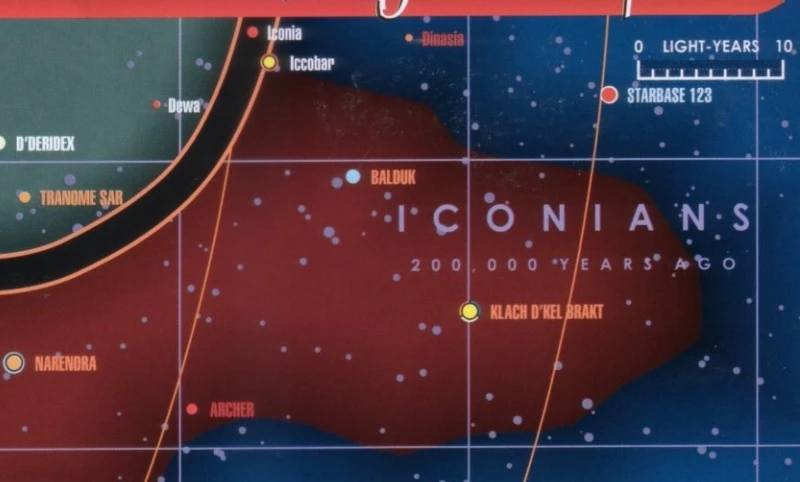
\includegraphics[width=1\linewidth]{img/Dinasia-Dewa-Iccobar.png}
\end{figure*}


\subsection{Eredità}
 

Gli Iconiani hanno lasciato rovine e artefatti sparsi per il quadrante. Molti di questi rimangono dormienti, ma contengono potenzialmente tecnologie che potrebbero rivoluzionare o destabilizzare l'equilibrio di potere galattico.

Diversi popoli moderni, come i Dewan, i Dinaali e gli Icoriani, rivendicano discendenze parziali dagli Iconiani, sebbene tali affermazioni siano difficili da verificare definitivamente.

La maggior parte delle conoscenze sugli Iconiani rimane teorica o dedotta da frammenti archeologici. La loro scrittura, composta da complessi simboli multidimensionali, resta in gran parte indecifrabile, aggiungendo un ulteriore velo di mistero a questa antica civiltà.

\section{La Shackleton Expanse}

La Shackleton Expanse rappresenta una delle regioni più enigmatiche e inesplorate del Quadrante Beta, un vasto territorio che si estende oltre i confini della Federazione Unita dei Pianeti e dello spazio klingon. Questa regione ha recentemente assunto importanza strategica e scientifica significativa, diventando un punto focale per l'esplorazione della Flotta Stellare.

\subsection{Geografia Stellare}

\begin{figure*}
    \centering
    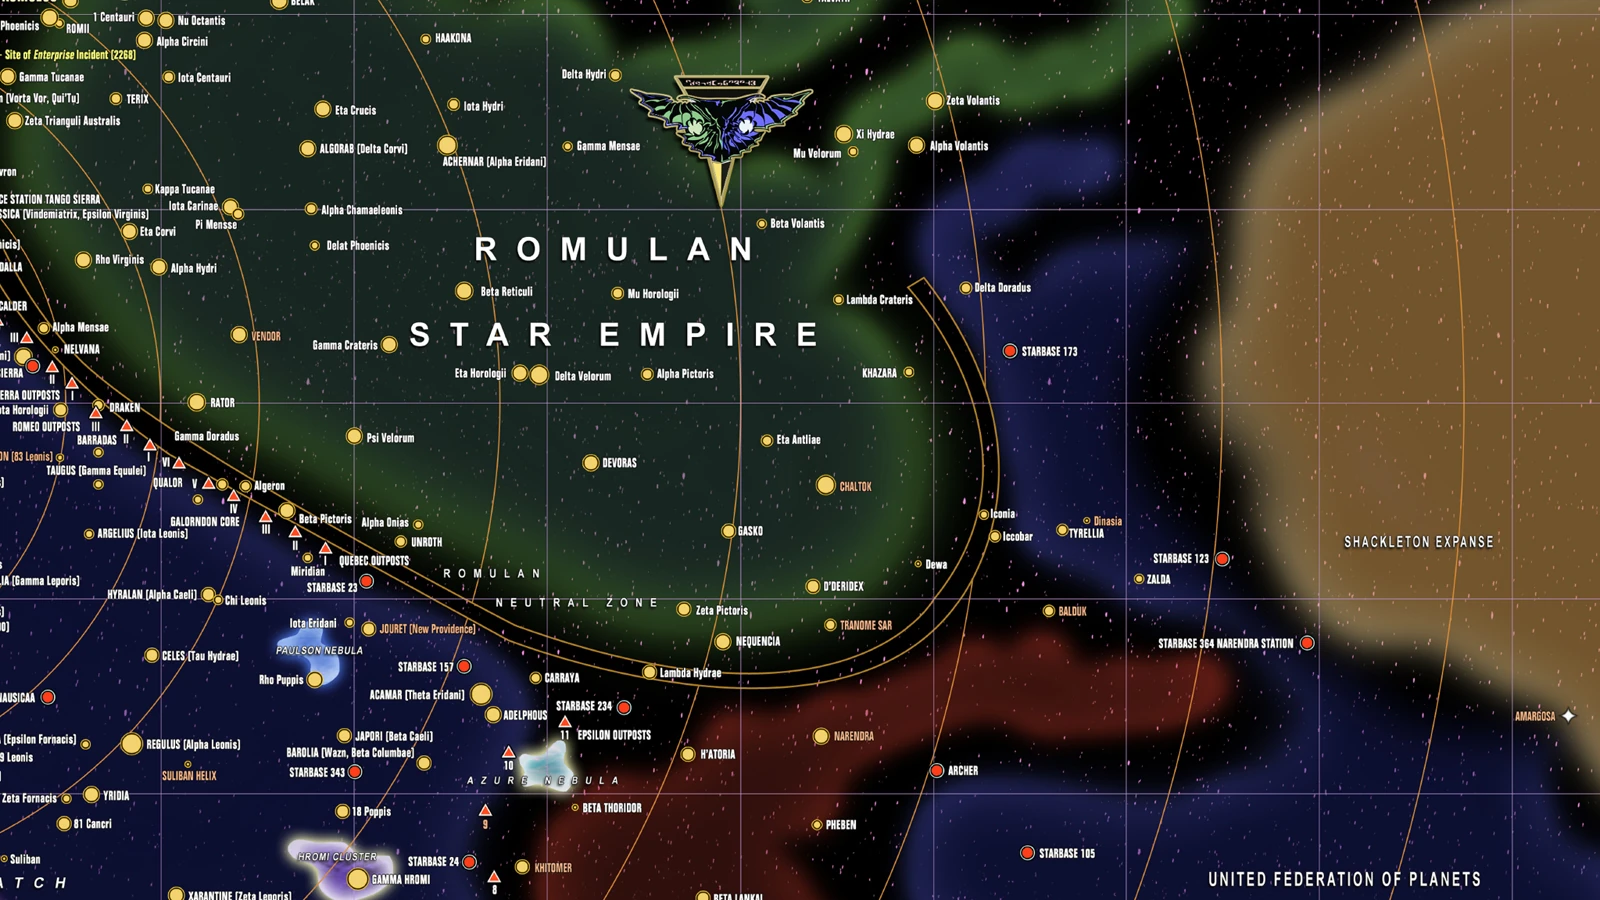
\includegraphics[width=1\linewidth]{img/Shackleton_vicinity.png}
\end{figure*}

La Shackleton Expanse copre un'area di circa 8 anni luce di diametro, caratterizzata da una densità stellare inferiore alla media galattica. Questa peculiarità crea "vuoti" interstellari che rendono la navigazione particolarmente complessa. Il settore contiene:

\begin{itemize}
    \item Diversi sistemi stellari binari e ternari con configurazioni orbitali instabili
    \item Numerose nebulose con proprietà ioniche uniche che interferiscono con i sensori
    \item Un insolito numero di stelle di neutroni e pulsar
    \item Zone di intensa radiazione tetrione che creano "bolle subspaziali"
\end{itemize}

La regione prende il nome dall'antico esploratore terrestre Ernest Shackleton, riflettendo le similarità tra l'esplorazione di questa zona spaziale e le pericolose spedizioni antartiche di Shackleton.

\subsection{Rilevanza Strategica}

La Shackleton Expanse occupa una posizione di cruciale importanza geopolitica, trovandosi all'intersezione di diverse sfere d'influenza:

\begin{itemize}
    \item Confina con i territori periferici della Federazione
    \item Si avvicina ai confini dell'Impero Klingon
    \item Contiene rotte potenziali verso il territorio romulano
    \item Include diversi mondi indipendenti con risorse significative
\end{itemize}

Questa posizione ha trasformato la regione in un "grande gioco" di diplomazia e influenza, con diverse potenze che cercano di stabilire avamposti e alleanze con le civiltà locali.

\subsection{Anomalie e Fenomeni}

La Shackleton Expanse è nota per l'alta concentrazione di anomalie subspaziali e fenomeni astrofisici:

\begin{itemize}
    \item "Maree subspaziali" che cambiano periodicamente le proprietà fisiche locali
    \item Anomalie temporali che causano occasionali "eco" di eventi passati o futuri
    \item Vortici gravitazionali che appaiono e scompaiono apparentemente senza causa
    \item Radiazioni quantiche non classificate che sembrano influenzare la materia in modi imprevedibili
\end{itemize}

Alcune di queste anomalie sembrano correlate a tecnologie antiche, incluse quelle iconiane, suggerendo che la regione potrebbe essere stata un tempo centrale per la civiltà iconiana.

\subsection{Civiltà e Insediamenti}

La Shackleton Expanse ospita diverse civiltà pre-curvatura e alcune specie che hanno recentemente sviluppato la tecnologia warp:

\begin{itemize}
    \item I Salorians, una specie anfibia che ha recentemente unificato il proprio pianeta
    \item I Xileth, una cultura nomade basata su enormi astronavi generazionali
    \item La Confederazione di Caldos, un'alleanza di colonie umane indipendenti
    \item Gli Atraxiani, una specie tecnologicamente avanzata ma estremamente isolazionista
\end{itemize}

Inoltre, la regione contiene diverse colonie indipendenti fondate da rifugiati e dissidenti di varie potenze maggiori, creando un ambiente politico complesso e frammentato.

\subsection{Stazione Narendra - Starbase 364}

Il principale punto di presenza della Federazione nella regione è Starbase 364\footnote{\url{https://memory-beta.fandom.com/wiki/Starbase_364}}, chiamata \textit{Stazione Narendra}, una stazione spaziale di classe Nomad situata ai margini della Shackleton Expanse. Questa stazione serve come:

\begin{itemize}
    \item Base avanzata per missioni di esplorazione
    \item Centro diplomatico per relazioni con le specie locali
    \item Hub scientifico per lo studio delle anomalie della regione
    \item Punto di coordinamento per le operazioni della Flotta Stellare
\end{itemize}

La stazione è comandata dall'Ammiraglio Hebert ed è stata recentemente potenziata con sistemi difensivi e scientifici avanzati in risposta alla crescente importanza strategica della regione.

\subsubsection{Personale di Narendra Station}
\paragraph{Ammiraglio Hebert}
\paragraph{Generale Kargan}
\paragraph{Eng. Olok}
\paragraph{Cmd. N'ria}
\paragraph{Dr. Helena Taliaferro}

\subsection{Segreti e Misteri}

La Shackleton Expanse è costellata di misteri che attendono di essere svelati:

\begin{itemize}
    \item Rovine di civiltà estinte che presentano tecnologie non classificabili
    \item Tracce di antichi conflitti di scala galattica
    \item Evidenze di esperimenti di terraformazione abbandonati
    \item Possibili portali o nodi di transito iconiani dormienti
\end{itemize}

Questi elementi, combinati con le anomalie naturali, rendono la regione una delle frontiere più promettenti e pericolose per l'esplorazione scientifica.

La natura largamente inesplorata della Shackleton Expanse la rende il luogo ideale per scoperte impreviste, incontri con nuove forme di vita e civiltà, e possibili rivelazioni sui segreti dell'antica civiltà iconiana, rendendo questa regione un perfetto scenario per avventure che combinano esplorazione, diplomazia e scoperta scientifica.

\section{La Coalizione dei Mondi Indipendenti della Shackleton Expanse}
\subsection{Origine e Formazione}
La Coalizione è nata circa tre decenni fa come risposta alla crescente influenza delle potenze maggiori (Federazione, Klingon, Romulani) nella regione della Shackleton Expanse. Inizialmente fondata da cinque colonie umane indipendenti che temevano di essere assorbite dall'espansione federale, ha gradualmente incorporato altri mondi di varie specie accomunati dal desiderio di autodeterminazione.
\subsection{Composizione Demografica}
La Coalizione è caratterizzata da un'eccezionale diversità:

\begin{itemize}
    \item \textbf{Umani Indipendenti}: Discendenti di coloni che lasciarono la Terra prima della formazione della Federazione o che si separarono successivamente per mantenere autonomia culturale e politica
    \item \textbf{Caldosiani}: Una popolazione umana geneticamente adattata ai mondi freddi e piovosi, sviluppando una cultura focalizzata sulla conservazione delle risorse
    \item \textbf{Veshi}: Specie anfibio-umanoide nativa della regione, con abilità telepatiche limitate e una profonda tradizione di navigazione stellare
    \item \textbf{Exofughi Tellariti}: Comunità separatiste che hanno abbandonato Tellar Prime in disaccordo con l'adesione alla Federazione
    \item \textbf{Rifugiati Romulani}: Un numero crescente di cittadini romulani che hanno cercato asilo dopo la catastrofe di Hobus, portando con sé competenze tecnologiche avanzate
\end{itemize}

\subsection{Struttura Politica}
La Coalizione è governata da un Consiglio dei Rappresentanti con sede su Caldos II, operante secondo un principio di consenso piuttosto che di votazione maggioritaria. Le decisioni vengono prese solo quando tutti i membri concordano, rendendo il processo decisionale lento ma stabile.
Il sistema politico è caratterizzato da:

\begin{itemize}
    \item Forte autonomia locale per ciascun mondo
    \item Difesa condivisa attraverso la Flotta di Difesa della Coalizione
    \item Politica commerciale comune verso potenze esterne
    \item Non-ingerenza nelle questioni culturali interne di ciascun mondo
\end{itemize}

\subsection{Tecnologia e Capacità Militari}
La tecnologia della Coalizione è un ibrido pragmatico di diverse influenze:

\begin{itemize}
    \item Sistemi propulsivi di derivazione umana ma modificati con principi energetici tellariti
    \item Scudi di protezione ispirati alle tecnologie romulane ma meno avanzati
    \item Sistemi di comunicazione quantica sviluppati autonomamente dai Veshi
    \item Strutture navali robuste ma meno sofisticate di quelle della Federazione
\end{itemize}

La HSS Ironclad rappresenta una delle navi più avanzate della Flotta di Difesa, progettata specificamente per operazioni autonome di lunga durata nelle regioni più remote della Shackleton Expanse.
\subsection{Cultura e Valori}
La cultura della Coalizione è definita da alcuni principi fondamentali:

\begin{itemize}
    \item Pragmatismo e autosufficienza come virtù primarie
    \item Diffidenza verso le grandi potenze e le loro promesse
    \item Forte etica dell'autodifesa e preparazione al peggio
    \item Valorizzazione del commercio e della cooperazione pratica
    \item Rispetto per le diverse tradizioni con minima interferenza
\end{itemize}

Una caratteristica distintiva delle comunità della Coalizione è il "Giuramento di Indipendenza" che ogni cittadino pronuncia al raggiungimento della maggiore età, promettendo di preservare l'autonomia dei propri mondi.
\subsection{Relazione con l'Artefatto Iconiano}
La Coalizione ha un interesse particolare nell'artefatto iconiano:

\begin{itemize}
    \item Rappresenta una potenziale minaccia se controllato da potenze maggiori
    \item Potrebbe offrire capacità difensive cruciali per garantire l'indipendenza a lungo termine
    \item È visto come un patrimonio della regione che non dovrebbe essere sfruttato da "invasori esterni"
    \item Alcuni leader credono che la tecnologia potrebbe finalmente livellare lo squilibrio di potere con la Federazione
    \item 
\end{itemize}
Il comandante della HSS Ironclad ha ordini di assicurarsi che l'artefatto non diventi uno strumento di dominio da parte di alcuna grande potenza, anche a costo di neutralizzarlo completamente.

\section{Europa Nova - Colonia Mineraria Umana Indipendente}
\subsection{Origine e Storia}
Europa Nova è stata fondata 78 anni fa come avamposto minerario da un consorzio di compagnie terrestri indipendenti, operanti al di fuori della giurisdizione della Federazione. Situata su un pianeta ricco di minerali nel sistema Tartarus, la colonia è cresciuta da un semplice avamposto estrattivo a una società complessa e autosufficiente. Quando il consorzio originale fallì durante la crisi economica del 2320, i coloni decisero di rimanere e dichiararono l'indipendenza, assumendo il controllo delle operazioni minerarie.
\subsection{Società e Popolazione}
La popolazione di Europa Nova (circa 38.000 persone) è composta principalmente da:

Minatori e tecnici specializzati
Ingegneri ambientali che mantengono le cupole abitative
Commercianti indipendenti
Discendenti di rifugiati delle Guerre Eugenetiche

La società è organizzata secondo un modello di "democrazia corporativa" dove i cittadini sono anche azionisti della Cooperativa Mineraria di Europa Nova. Le decisioni vengono prese attraverso votazioni ponderate in base a competenze specifiche e anni di servizio, non per ricchezza personale.
\subsection{Caratteristiche Culturali}
La cultura di Europa Nova è profondamente influenzata dall'ambiente minerario e dalla storia di autodeterminazione:

\begin{itemize}
    \item Forte etica del lavoro e valorizzazione delle competenze pratiche
    \item Tradizione di auto-governance e sospetto verso autorità esterne
    \item "Cerimonia dell'Estrazione" annuale che celebra la fondazione della colonia
    \item Codice d'onore che enfatizza l'autosufficienza e la responsabilità comunitaria
    \item Adattamenti culturali specifici alla vita in un ambiente ostile (riti di gestione della clausura, segnali non verbali per comunicare in condizioni pericolose)
\end{itemize}

\subsection{Tecnologia e Risorse}
Europa Nova ha sviluppato tecnologie specifiche adattate alle proprie necessità:

\begin{itemize}
    \item Avanzati sistemi di perforazione e estrazione mineraria
    \item Tecnologia di fusione compatta per le operazioni remote
    \item Scanner geologici di precisione superiore a quelli federali standard
    \item Sistemi di supporto vitale efficienti progettati per funzionare in ambienti estremi
    \item La nave SS Halcyon, originariamente una nave cargo modificata con capacità di estrazione specializzate
    \item 
\end{itemize}
Le principali risorse estratte includono:

\begin{itemize}
    \item Dilithio ad alta purezza
    \item Elementi delle terre rare
    \item Benamite (cruciale per motori a curvatura avanzati)
    \item Duranium e tritanium per costruzioni spaziali
\end{itemize}
\subsection{Relazioni Esterne}
Europa Nova mantiene una posizione di neutralità pragmatica:

\begin{itemize}
    \item Commercia con la Federazione ma mantiene l'indipendenza politica
    \item Ha accordi commerciali non esclusivi con i Ferengi
    \item Evita coinvolgimenti con l'Impero Klingon e l'Impero Stellare Romulano
    \item Mantiene relazioni cordiali ma distanti con la Coalizione dei Mondi Indipendenti
    \item Ha sviluppato un network di commercianti indipendenti fidati
\end{itemize}

\subsection{Interesse nell'Artefatto Iconiano}
L'interesse di Europa Nova nell'artefatto si basa su motivazioni pratiche:

\begin{itemize}
    \item L'anomalia subspaziale ha inizialmente attratto l'attenzione per le sue strane letture energetiche, simili a depositi minerari ad alta concentrazione
    \item I colonisti sono preoccupati per potenziali rischi per il pianeta e le operazioni minerarie
    \item Alcuni anziani considerano l'artefatto una potenziale fonte di tecnologia che potrebbe rivoluzionare le tecniche minerarie
    \item C'è una legittima preoccupazione che l'artefatto possa attirare attenzione indesiderata da potenze maggiori nella regione di Europa Nova
\end{itemize}

L'equipaggio della SS Halcyon è stato inviato per valutare sia il potenziale sfruttamento sia i possibili rischi dell'artefatto, con una preferenza per soluzioni che garantiscano la sicurezza della colonia a lungo termine, anche a costo di opportunità economiche immediate.

\chapter{Schematiche}
\section{ Nave Stellare Classe Nova}

La Classe Nova rappresenta una delle navi scientifiche più avanzate della Flotta Stellare, progettata specificamente per missioni di ricerca e esplorazione dettagliata. Considerevolmente più piccola delle navi principali della flotta come la Galaxy o la Sovereign, la Nova eccelle in indagini scientifiche specializzate.

\subsection{Specifiche Tecniche:}
\begin{itemize}
    \item \textbf{Lunghezza}: circa 165 metri
    \item \textbf{Equipaggio}: 80-85 membri
    \item \textbf{Velocità massima}: Curvatura 8
    \item \textbf{Armamento}: Limitato ma presente (phaser di tipo X, tubi lanciasiluri)
    \item \textbf{Peso}: Approssimativamente 110.000 tonnellate metriche
\end{itemize}

\subsection{ Caratteristiche Distintive:}
\begin{itemize}
    \item Design compatto con i gondoloni di curvatura integrati direttamente nello scafo primario
    \item Sezione a disco molto appiattita rispetto alle navi più grandi
    \item Sistemi sensoriali all'avanguardia particolarmente adatti per scansioni planetarie e analisi dettagliate
    \item Laboratori scientifici specializzati che occupano una porzione significativa degli spazi interni
\end{itemize}

\subsection{ Funzione:}
Le navi classe Nova sono progettate principalmente per missioni scientifiche di ricognizione avanzata, analisi planetaria, ricerca astronomica e indagini su fenomeni stellari. Non sono concepite per funzioni diplomatiche estese o per missioni di combattimento prolungato, ma la loro velocità e manovrabilità le rende efficaci nelle missioni di esplorazione in cui potrebbe essere necessario raccogliere dati dettagliati in tempi relativamente brevi.

La USS Venture, come nave di classe Nova, possiede quindi capacità scientifiche superiori alla media che sarebbero particolarmente utili nello studio dell'artefatto iconiano, ma probabilmente si trova in svantaggio tattico rispetto alla nave romulana nel caso di un confronto diretto.

\begin{figure*}
    \centering
    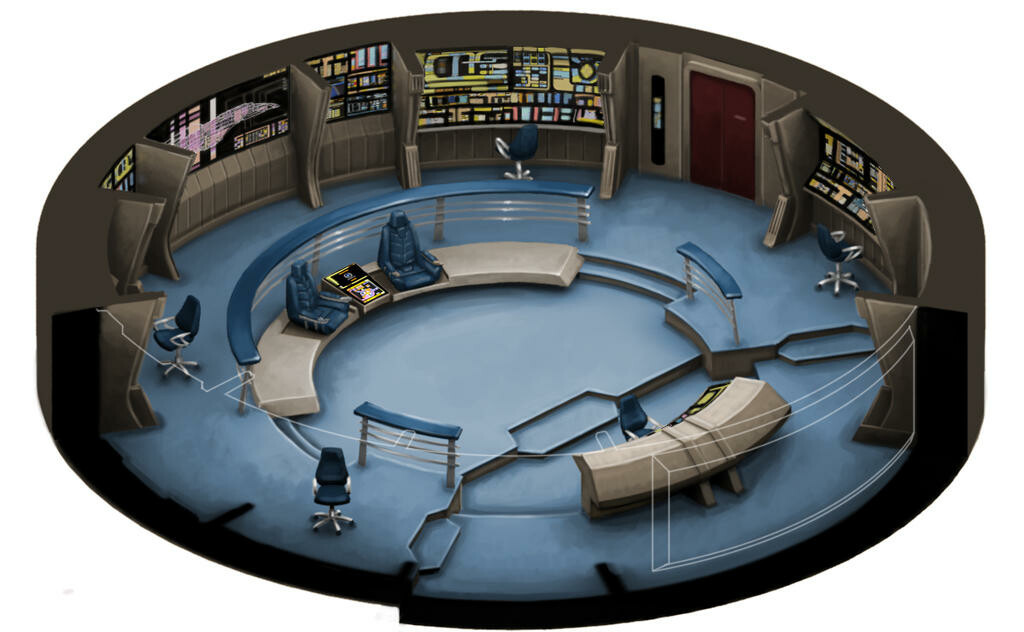
\includegraphics[width=1\linewidth]{img/wayne-peters-nova-bridge-painting-by-scarecrovv-dc1qvhn-fullview.jpg}
    \caption{Ponte della classe Nova - isometrico}
    \label{fig:enter-label}
\end{figure*}
\begin{figure*}
    \centering
    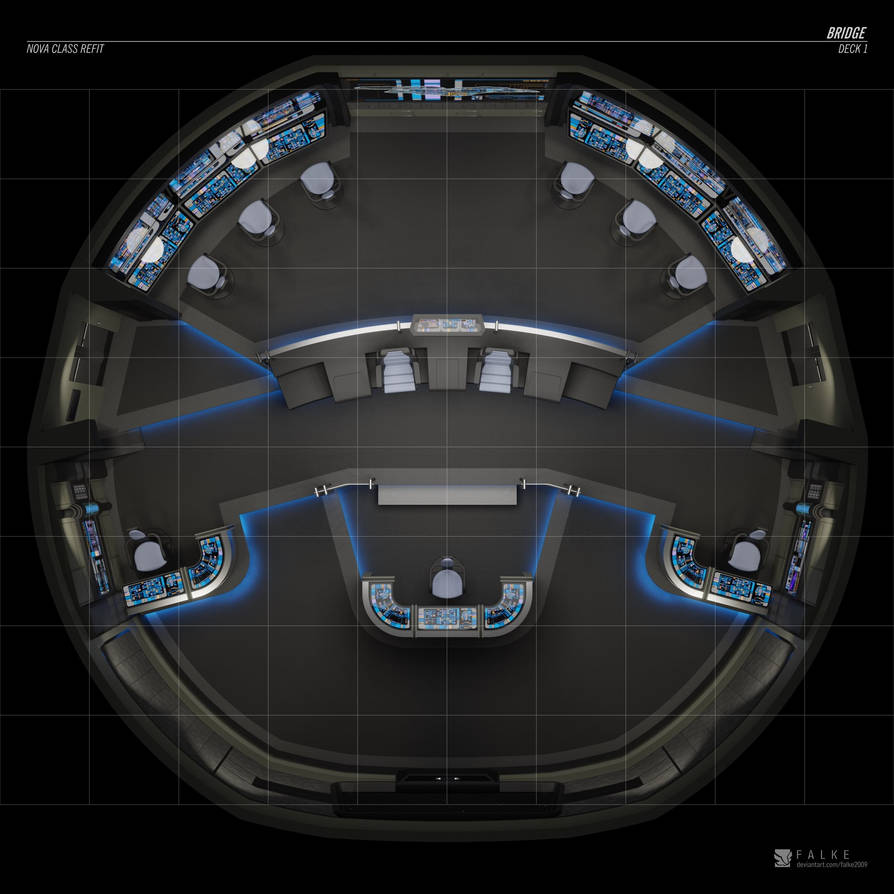
\includegraphics[width=1\linewidth]{img/bridge_tile_01__1___1__by_captain_harker_deyxp3i-pre (1).jpg}
    \caption{Ponte della classe Nova - battlegrid}
    \label{fig:enter-label}
\end{figure*}

\section{Nave scientifica romulana - Classe Tal'Aura}

\subsection{ Descrizione Generale}
La Tal'Aura è una delle classi più recenti di vascelli scientifici romulani, sviluppata nel periodo post-Hobus quando l'Impero dovette ripensare le proprie priorità. Prende il nome da un importante leader politico del periodo di transizione e rappresenta il desiderio romulano di ricostruire attraverso conoscenza e innovazione, piuttosto che solo attraverso potenza militare.

\subsection{ Specifiche Tecniche:}
\begin{itemize}
    \item \textbf{Lunghezza}: circa 320 metri
    \item \textbf{Equipaggio}: 200-250 (con alta percentuale di personale scientifico)
    \item \textbf{Velocità massima}: Curvatura 9.7
    \item \textbf{Armamento}: Medio (disruptori di precisione, siluri al plasma in numero limitato)
    \item \textbf{Occultamento}: Sistema di occultamento di nuova generazione che richiede meno energia
\end{itemize}

\subsection{ Caratteristiche Scientifiche:}
\begin{itemize}
    \item Laboratori specializzati in archeologia e tecnologia antica
    \item Sensori quantici ad alta risoluzione progettati per analisi di artefatti
    \item Suite di ingegneria inversa per lo studio di tecnologie sconosciute
    \item Capacità di estrazione e contenimento di energia subspaziale
    \item Bay scientifica modulare adattabile a vari tipi di missione
\end{itemize}

\subsection{ Considerazioni Tattiche:}
Il design mantiene elementi estetici romulani riconoscibili ma più eleganti e funzionali, con ali più corte e uno scafo più aerodinamico. La nave è progettata per operare per lunghi periodi in missioni scientifiche indipendenti, riflettendo la necessità dell'Impero di espandere la propria conoscenza per ricostruire dopo la catastrofe di Hobus.

\begin{figure*}
    \centering
    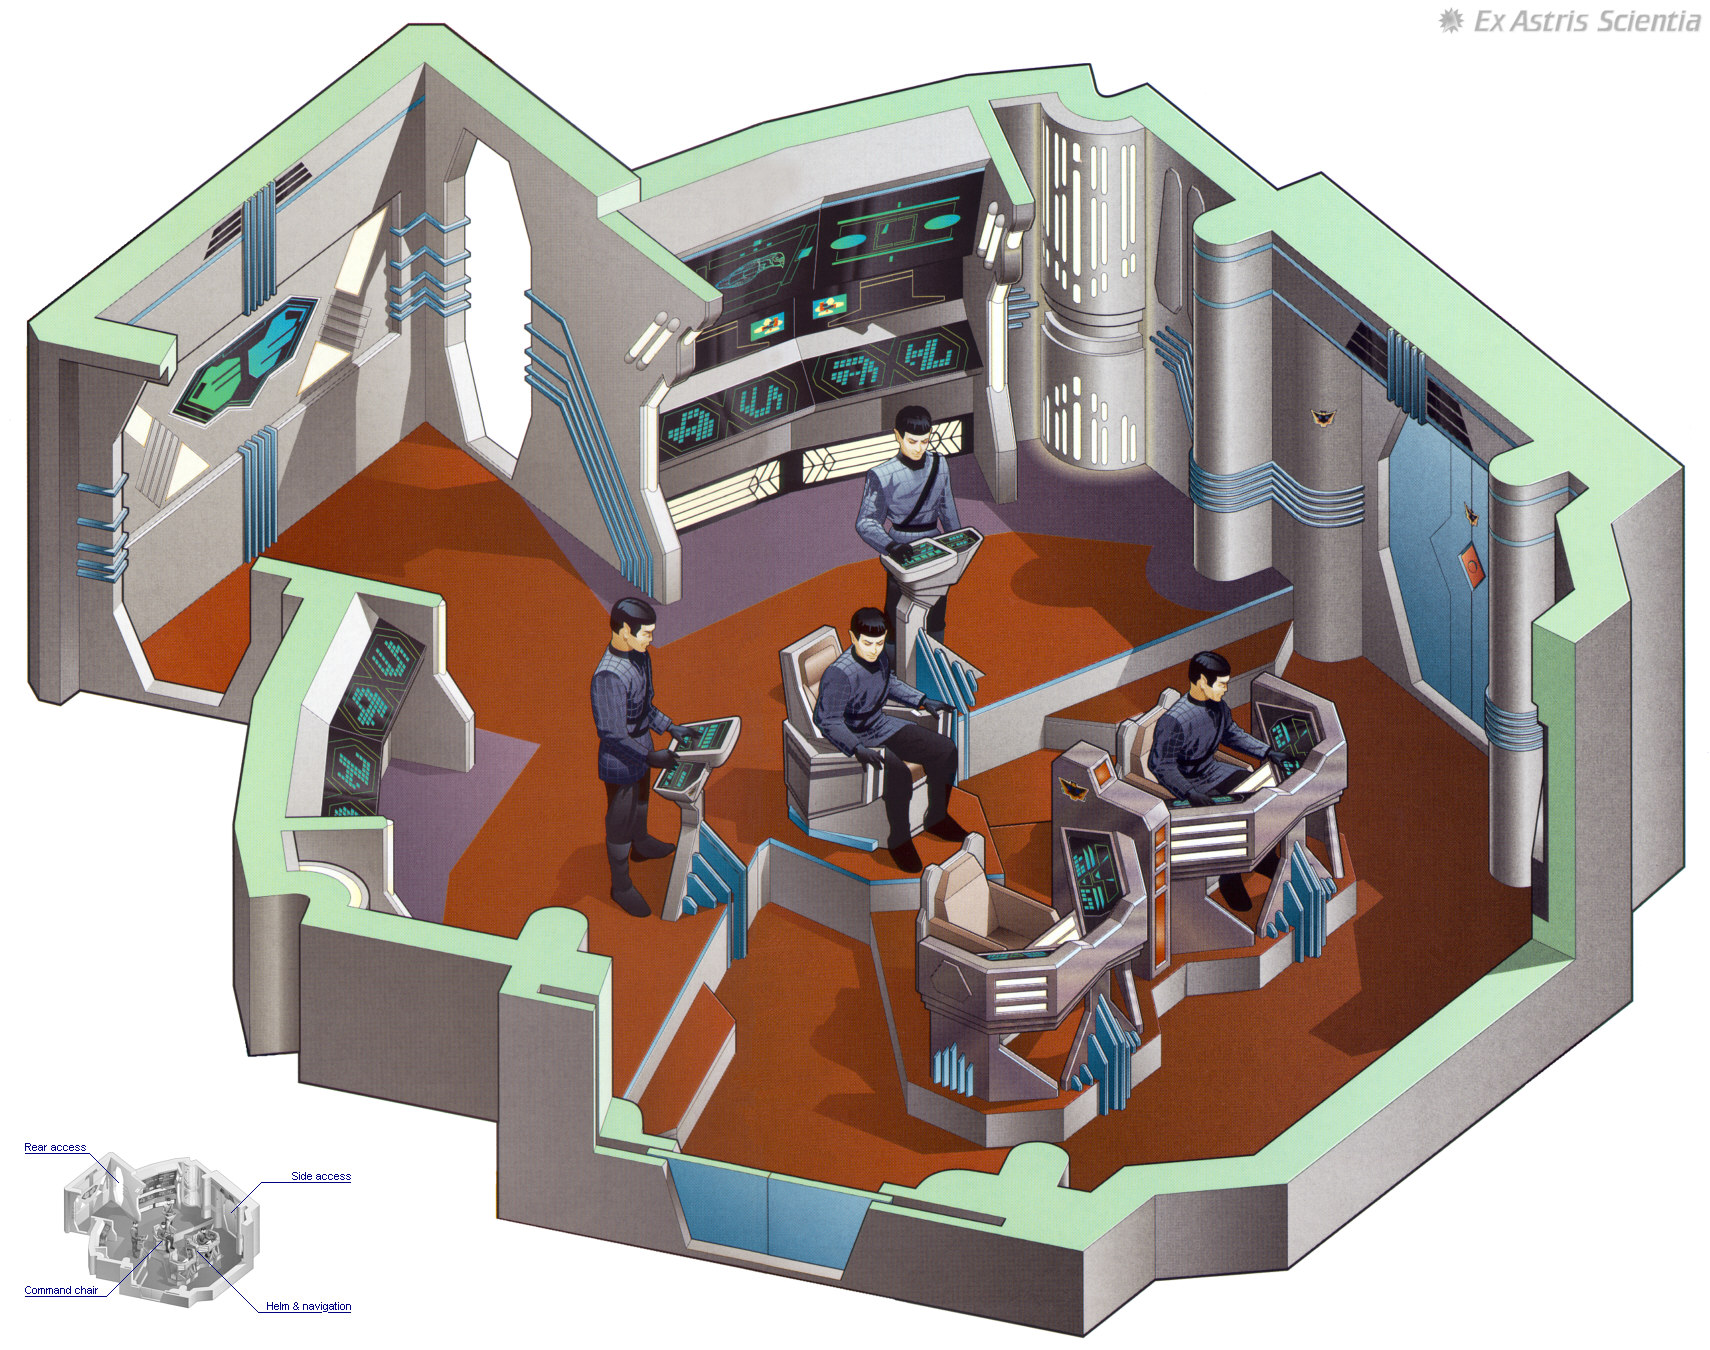
\includegraphics[width=1\linewidth]{img/warbird-bridge.jpg}
    \caption{Ponte di nave class Tal'Aura - isometrica}
    \label{fig:enter-label}
\end{figure*}


\end{document}

